\documentclass[11pt,a4paper]{article}

\usepackage[margin=1in]{geometry}
\usepackage[T1]{fontenc}
\usepackage[utf8]{inputenc}
\usepackage{graphicx}
\usepackage{booktabs}
\usepackage{array}
\usepackage{longtable}
\usepackage{enumitem}
\usepackage{xcolor}
\usepackage{titlesec}
\usepackage{float}
\usepackage[colorlinks=true,linkcolor=black,citecolor=blue,urlcolor=blue]{hyperref}

\setlength{\parindent}{0pt}
\setlength{\parskip}{0.7em}
\setlist[itemize]{leftmargin=1.5em}
\setlist[enumerate]{leftmargin=1.8em}

\titleformat{\section}
  {\Large\bfseries}
  {\thesection}
  {0.75em}
  {}

\titleformat{\subsection}
  {\large\bfseries}
  {\thesubsection}
  {0.75em}
  {}

\title{Progress Report: Prostate Lesion Segmentation}
\author{Ramal Salha}
\date{\today}

\begin{document}

\maketitle
\tableofcontents
\newpage

\section{Introduction and Thesis Topic}

This report summarizes the work completed so far on my master's thesis about automatic segmentation of suspicious prostate lesions from MRI data. The goal of the thesis is to develop and evaluate deep learning models that can segment lesion regions from prostate MRI in a reliable and interpretable way.

In this work I focused on multimodal prostate MRI, mainly T2w, ADC, and HBV images. So far, I prepared the training pipeline, tested several model families, evaluated multiple runs, generated qualitative visualizations, and performed explainable AI analysis.

\subsection{Main Goal}

Systems that enable fast and accurate detection and quantification of prostate tumor lesions are important in clinical practice because they can improve both the speed and the consistency of diagnosis. The main goal of this thesis is to develop and evaluate a method for automatic segmentation of suspicious prostate lesions from MRI data.

The work is based on multimodal prostate MRI, mainly T2-weighted, ADC, and HBV/DWI images. The approach relies on deep learning segmentation models together with preprocessing steps such as normalization, registration, and multimodal input preparation.

So far, I implemented the training and evaluation pipeline, tested several model families, compared multiple training runs, generated qualitative visualizations, and performed explainable AI analysis to better understand model behavior.

\section{Technical Overview}

This section gives a short overview of the implemented pipeline and the main experimental setup used so far.

\subsection{Pipeline Overview}

The workflow starts with loading prostate MRI volumes and their corresponding lesion masks, followed by preprocessing steps such as normalization, registration, and preparation of multimodal input data. The models are then trained for binary lesion segmentation using one or more MRI modalities, depending on the experiment. During training, validation is used to monitor model quality and to compare different runs. After training, the selected checkpoints are evaluated on the test set, and additional qualitative visualizations and explainable AI outputs are generated.

\subsection{Implemented Model Families}

Three main model families were tested in this work. Attention U-Net 3D was used as a strong convolutional baseline for multimodal medical image segmentation. Deconver was included as a newer medical segmentation architecture based on deconvolutional feature mixing \cite{deconver}. FCT was tested as a transformer-based comparison model in order to evaluate a different architectural approach \cite{fct}, with convolutional-transformer context aligned with CvT-style design ideas \cite{cvt}.

\subsection{Evaluation Metrics}

The main metrics used during evaluation are composite score, Dice, IoU, sensitivity, precision, and HD95. In practice, Dice and IoU describe overlap quality between predicted and ground-truth lesions, sensitivity shows how well positive lesions are detected, precision measures how many predicted lesions are correct, and HD95 gives information about boundary quality. These metrics were used to compare the behavior of different runs and model families.

\subsection{Hardware and Training Setup}

The experiments were prepared and tested locally, while longer training runs were mainly executed in a Docker-based server environment. The models were trained on multimodal prostate MRI inputs, mainly T2w, ADC, and HBV images. The goal of this setup was to keep the training pipeline reproducible while allowing comparison of several architectures under similar conditions.

\section{Dataset}

This work mainly uses the PI-CAI public dataset for supervised prostate lesion segmentation \cite{picai_dataset}. The dataset contains prostate MRI volumes together with lesion annotations and was used as the main source of labeled data for training and evaluation.

\begin{table}[H]
\centering
\begin{tabular}{>{\raggedright\arraybackslash}p{0.42\textwidth} >{\raggedright\arraybackslash}p{0.42\textwidth}}
\toprule
Property & Value \\
\midrule
Dataset name & PI-CAI \\
Total cases & 1500 \\
Positive cases & 425 \\
Negative cases & 1075 \\
Modalities & T2w, ADC, HBV \\
Task & Binary lesion segmentation \\
\bottomrule
\end{tabular}
\caption{Short summary of the main supervised dataset.}
\end{table}

The dataset includes multimodal MRI acquisitions, where T2w provides anatomical information, while ADC and HBV provide functional information relevant for lesion detection. Lesion masks are treated as binary segmentation targets, where lesion voxels are separated from background voxels.

A fixed PI-CAI test set consisting of 10 cases, including 5 positive and 5 negative cases, was separated from the rest of the dataset and was never used during training or validation. As a result, training and validation were performed on the remaining 1490 PI-CAI cases.

In addition to this fixed PI-CAI test set, all runs were also evaluated on 19 Prostate158 test cases in order to check how the models behave on an additional external dataset \cite{prostate158_main}. Prostate158 data was also prepared and used as supporting data for related experiments such as pretraining and additional development work, and the dataset release details were documented in a companion data article \cite{prostate158_dib}.

\section{Experimental Work by Model Family}

This section groups runs by model family. Each subsection should start with a short explanation of why that model was tested and what kind of changes were explored.

\subsection{Attention U-Net 3D Runs}

Attention U-Net 3D was used as the main convolutional baseline for multimodal lesion segmentation. Several runs were performed in order to study the effect of loss weighting, checkpoint selection strategy, validation setup, patch size, and later also pretrained encoder initialization. Over time, these runs moved from high-sensitivity but unstable predictions toward more balanced segmentation results and stronger test performance. For each run, results are reported both on the fixed 10-case PI-CAI test set and on the 19-case Prostate158 test set.

\begin{table}[H]
\centering
\scriptsize
\begin{tabular}{>{\raggedright\arraybackslash}p{0.16\textwidth} >{\raggedright\arraybackslash}p{0.19\textwidth} c c c c c c}
\toprule
Run & Main change & P-Dice & P-Sens. & P-HD95 & Pr-Dice & Pr-Sens. & Pr-HD95 \\
\midrule
Attention baseline 1 & repeated early baseline & 0.2306 & 0.7699 & 174.3303 & 0.3858 & 0.5375 & 51.1937 \\
Attention baseline 2 & early high-sensitivity baseline & 0.1291 & \textbf{0.9552} & 181.4493 & 0.2683 & \textbf{0.8307} & 52.0160 \\
Attention baseline 3 & reduced BCE weight and HD95 validation & 0.5914 & 0.6959 & 70.5337 & \textbf{0.4726} & 0.5291 & 21.5574 \\
Attention baseline 4 & delayed validation start & 0.4731 & 0.8639 & 146.2934 & 0.4087 & 0.4714 & 38.2646 \\
Attention baseline 5 & reduced patch depth to 16 & 0.4864 & 0.7604 & 130.5286 & 0.4469 & 0.4659 & 31.7644 \\
Attention SSL run & SSL encoder init and larger feature sizes & \textbf{0.6332} & 0.8329 & \textbf{4.4875} & 0.4254 & 0.4948 & \textbf{18.6497} \\
\bottomrule
\end{tabular}
\caption{Attention U-Net 3D runs. P = PI-CAI 10-case test set, Pr = Prostate158 19-case test set.}
\normalsize
\end{table}

\subsubsection*{Detailed Run: Attention Baseline 2}

This run represents the early Attention U-Net baseline. The main goal was to establish a strong multimodal starting point using T2w, ADC, and HBV inputs. Compared to later runs, it used stronger BCE weighting, emphasized sensitivity in checkpoint selection, and did not include HD95 during training-time validation.

\begin{table}[H]
\centering
\begin{tabular}{lcc}
\toprule
Metric & PI-CAI (10 cases) & Prostate158 (19 cases) \\
\midrule
Dice & 0.1291 & 0.2683 \\
IoU & 0.0710 & 0.1731 \\
Sensitivity & 0.9552 & 0.8307 \\
Precision & 0.0715 & 0.1805 \\
HD95 & 181.4493 & 52.0160 \\
\bottomrule
\end{tabular}
\caption{Evaluation results for Attention baseline 2 on both test sets.}
\end{table}

\begin{figure}[H]
\centering
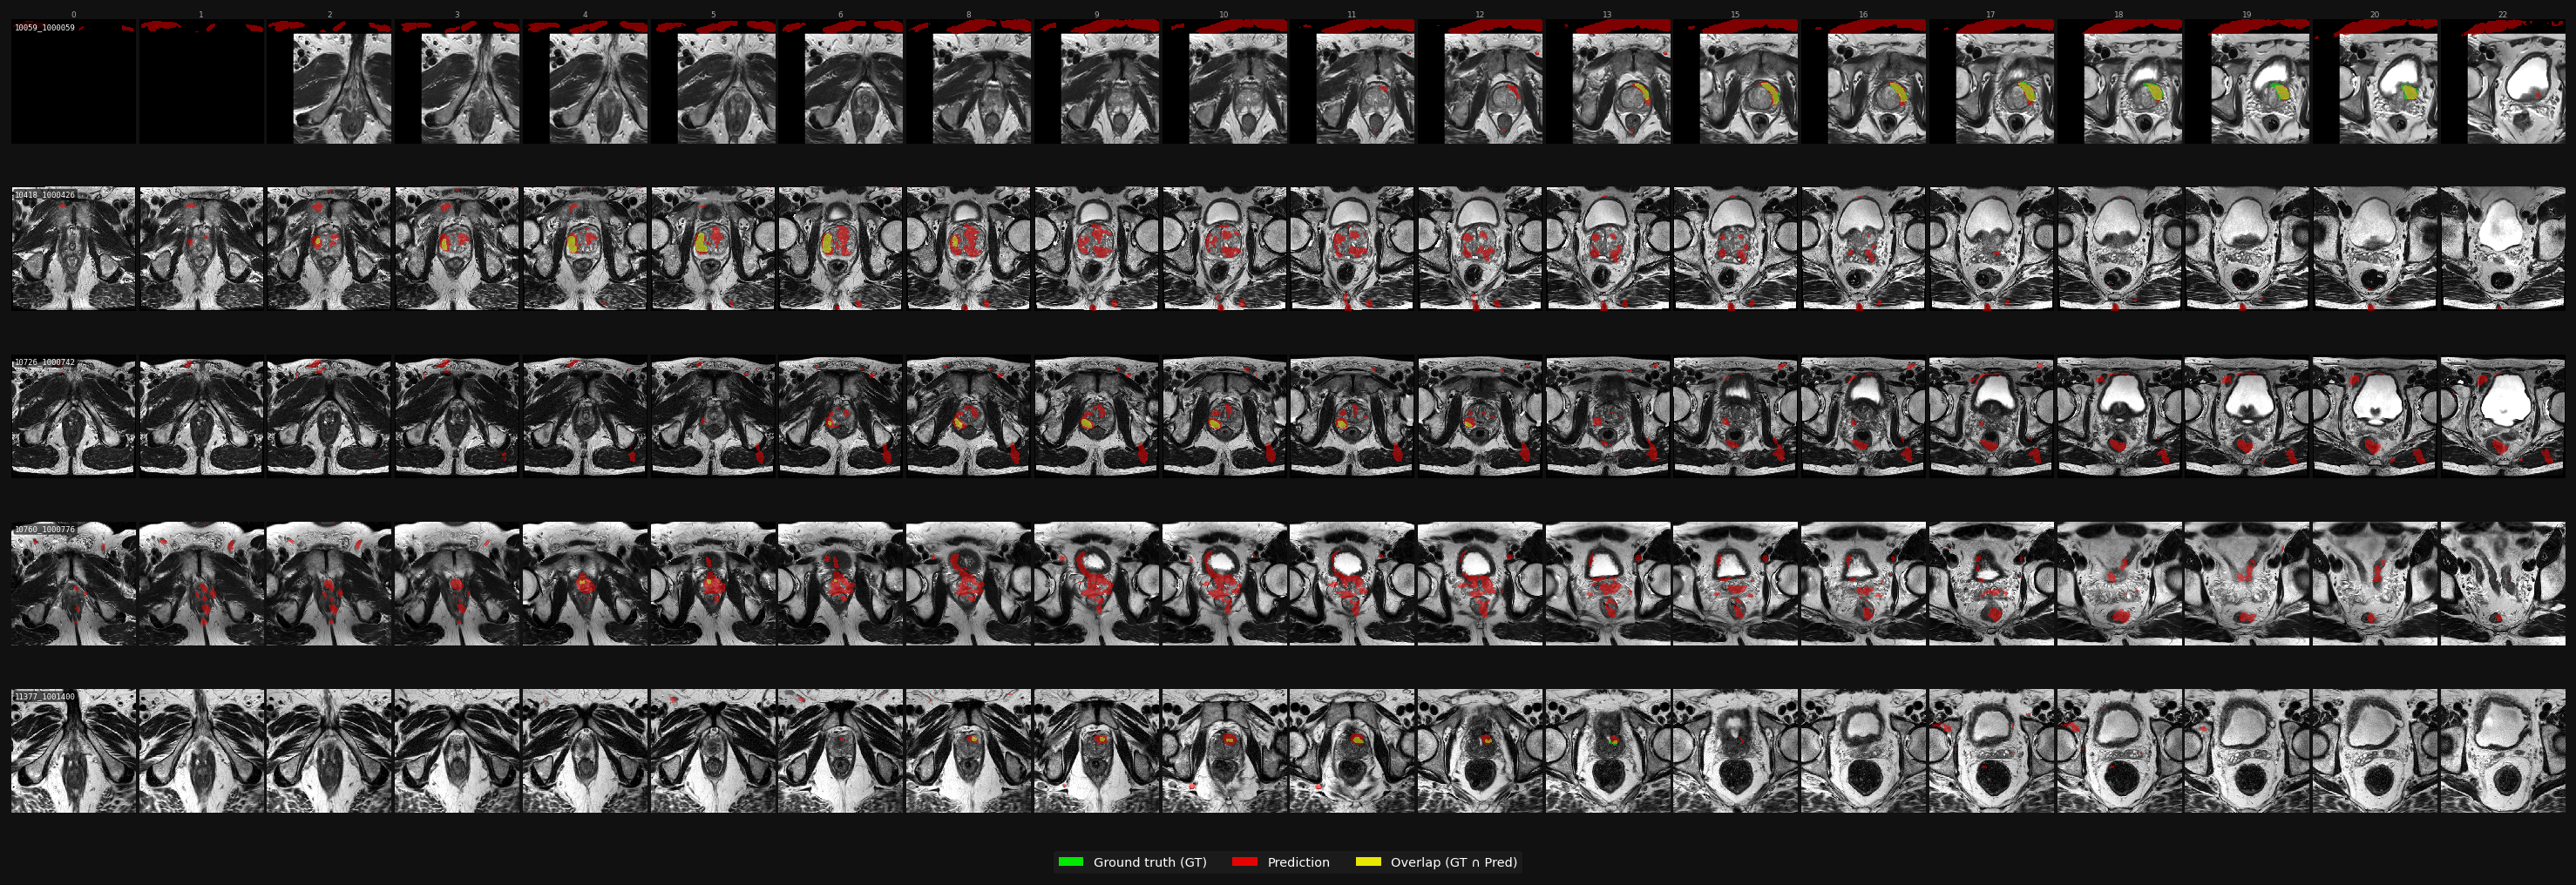
\includegraphics[width=0.78\textwidth]{../visualizations/20260415_210631_v3_multimodal_eval_visualization.png}
\caption{Example qualitative result for Attention baseline 2.}
\end{figure}

\begin{figure}[H]
\centering
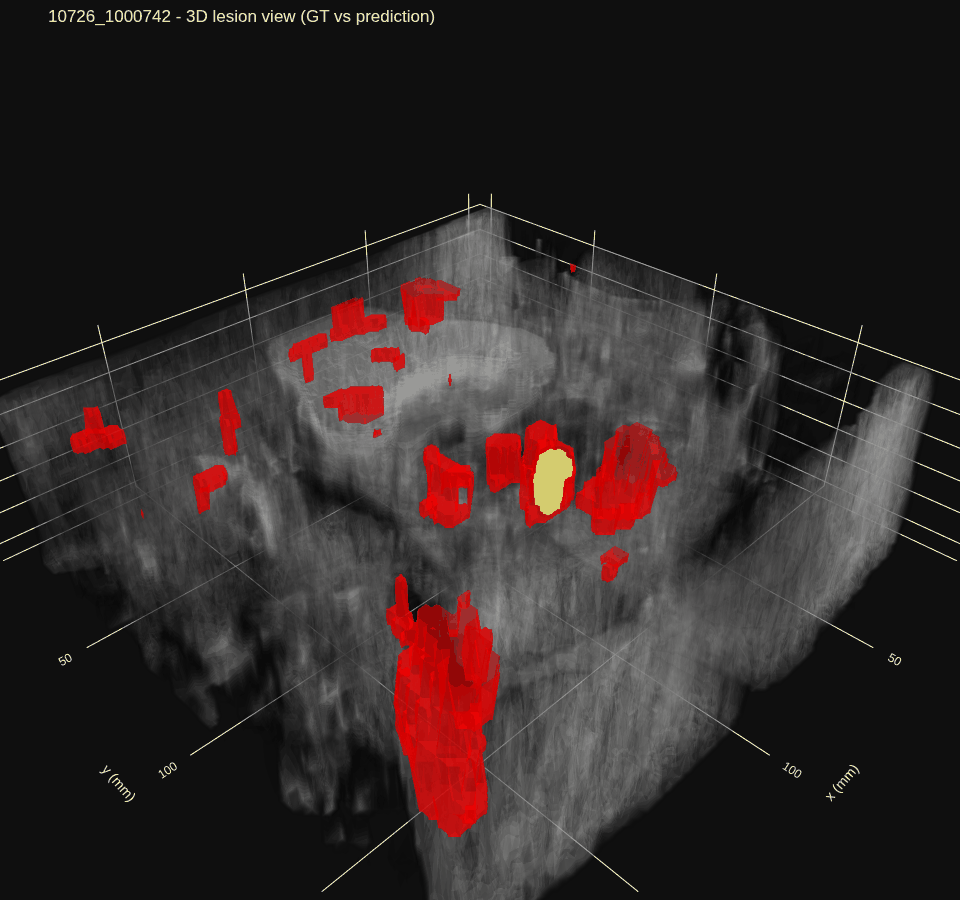
\includegraphics[width=0.78\textwidth]{../visualizations/20260415_210631_v3_multimodal_10726_1000742_t2w_orbit_first_frame.png}
\caption{Example 3D visualization for Attention baseline 2.}
\end{figure}

\subsubsection*{Detailed Run: Attention Baseline 3}

This run represents a more balanced Attention U-Net configuration. The main changes were lower BCE positive weighting, inclusion of HD95 during validation, and a checkpoint score that placed more emphasis on Dice than the earlier setup. The goal was to reduce oversegmentation and improve the overall quality of the predicted masks.

\begin{table}[H]
\centering
\begin{tabular}{lcc}
\toprule
Metric & PI-CAI (10 cases) & Prostate158 (19 cases) \\
\midrule
Dice & 0.5914 & 0.4726 \\
IoU & 0.4425 & 0.3499 \\
Sensitivity & 0.6959 & 0.5291 \\
Precision & 0.5456 & 0.5459 \\
HD95 & 70.5337 & 21.5574 \\
\bottomrule
\end{tabular}
\caption{Evaluation results for Attention baseline 3 on both test sets.}
\end{table}

\begin{figure}[H]
\centering
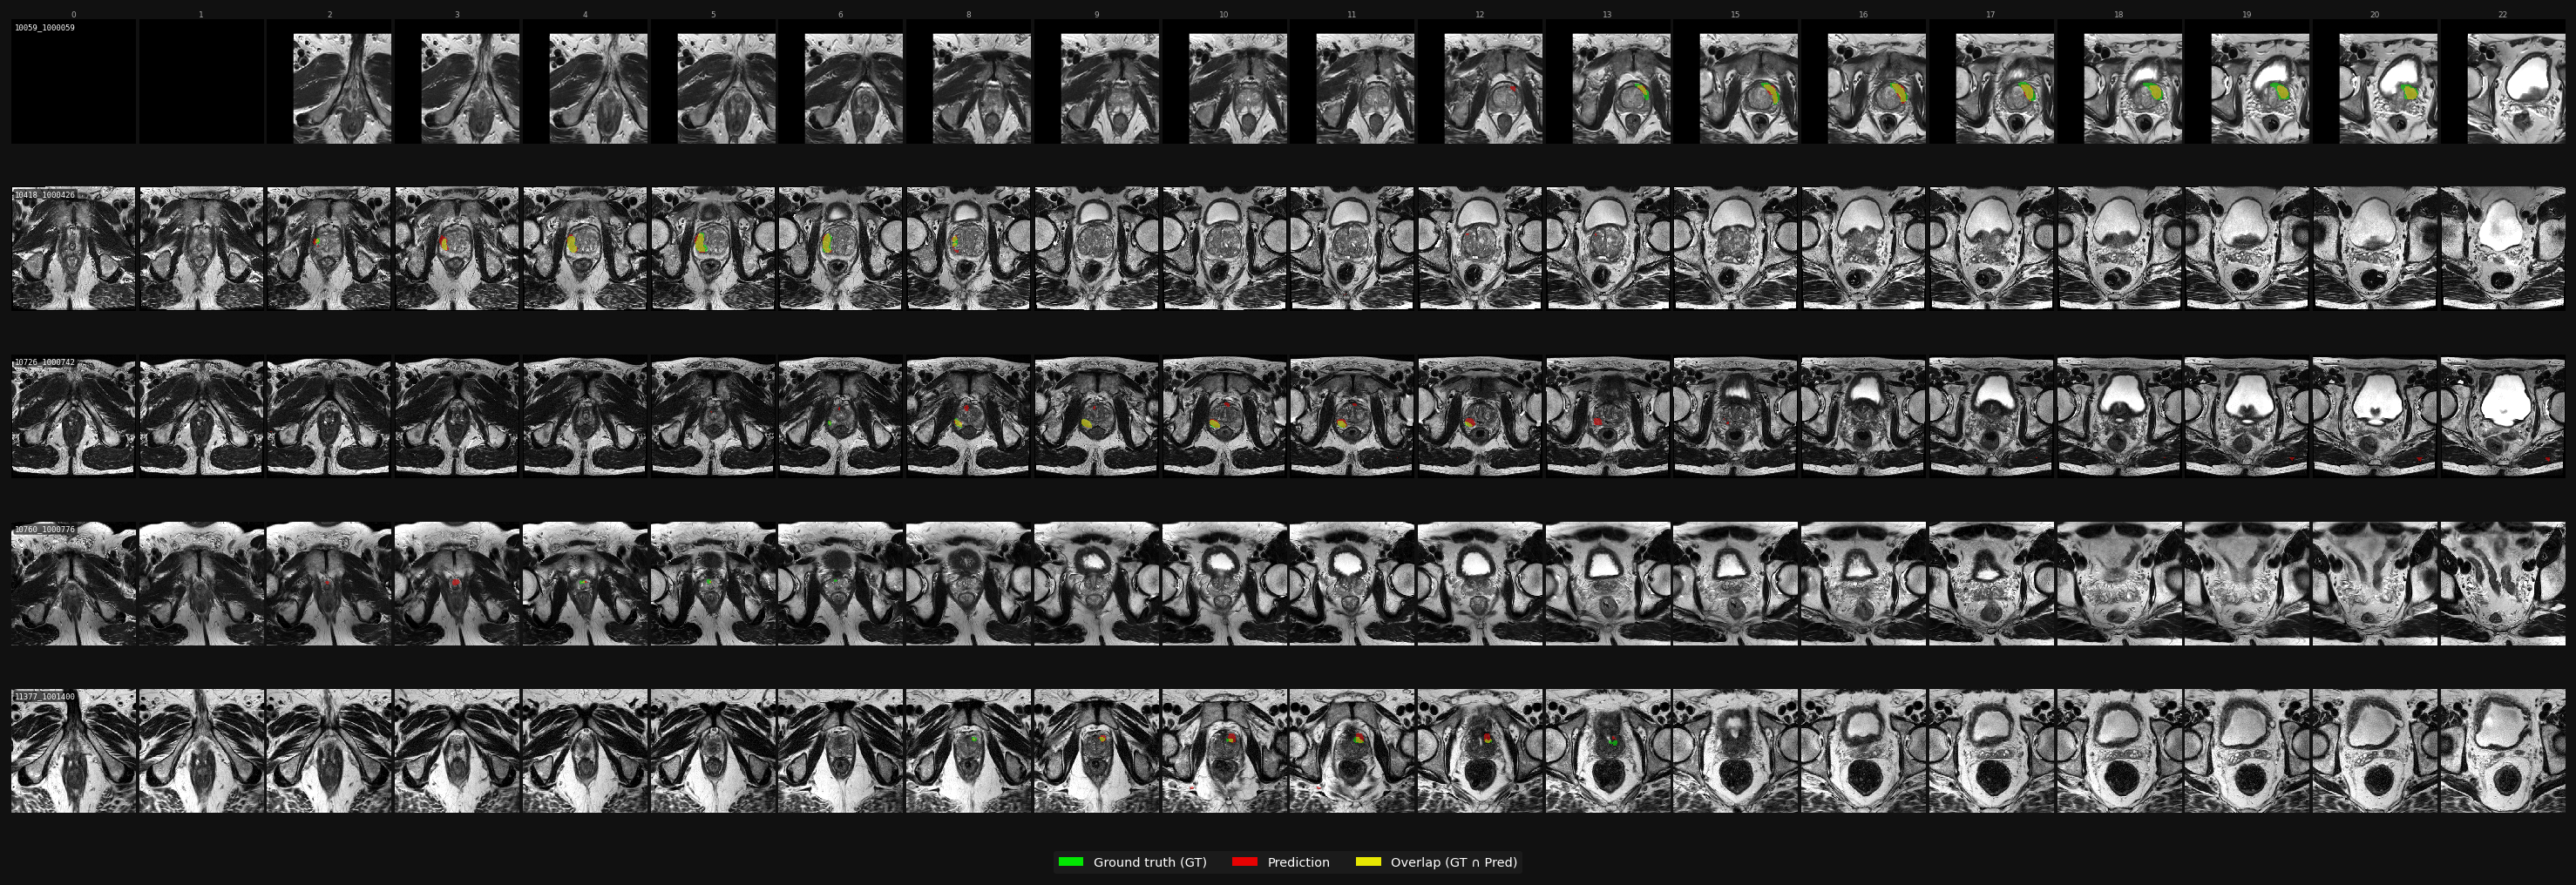
\includegraphics[width=0.78\textwidth]{../visualizations/20260416_112700_v3_multimodal_eval_visualization.png}
\caption{Example qualitative result for Attention baseline 3.}
\end{figure}

\begin{figure}[H]
\centering
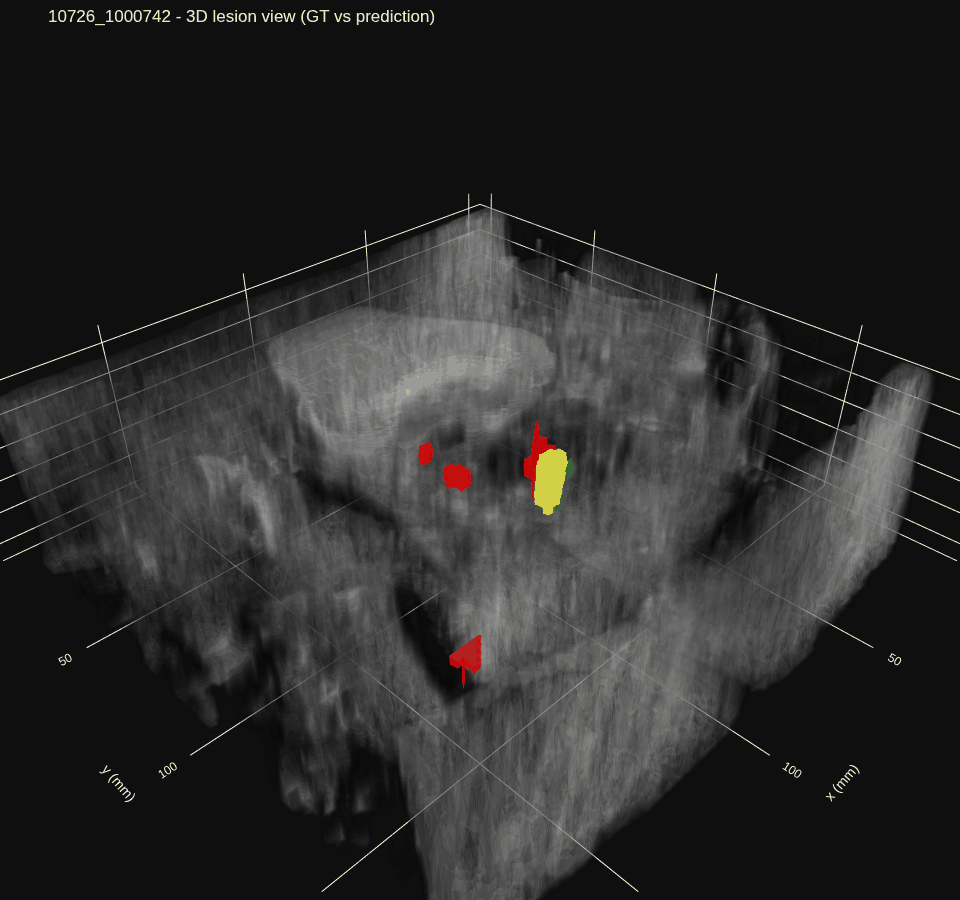
\includegraphics[width=0.78\textwidth]{../visualizations/20260416_112700_v3_multimodal_10726_1000742_t2w_orbit_first_frame.png}
\caption{Example 3D visualization for Attention baseline 3.}
\end{figure}

\subsubsection*{Detailed Run: Attention SSL Run}

This run was the strongest Attention U-Net variant on the fixed PI-CAI test set. It used a larger feature configuration together with pretrained encoder initialization from SSL pretraining. The goal was to test whether a stronger encoder and transferred representation could improve segmentation quality.

\begin{table}[H]
\centering
\begin{tabular}{lcc}
\toprule
Metric & PI-CAI (10 cases) & Prostate158 (19 cases) \\
\midrule
Dice & 0.6332 & 0.4254 \\
IoU & 0.4820 & 0.3208 \\
Sensitivity & 0.8329 & 0.4948 \\
Precision & 0.5876 & 0.5517 \\
HD95 & 4.4875 & 18.6497 \\
\bottomrule
\end{tabular}
\caption{Evaluation results for the Attention SSL run on both test sets.}
\end{table}

\begin{figure}[H]
\centering
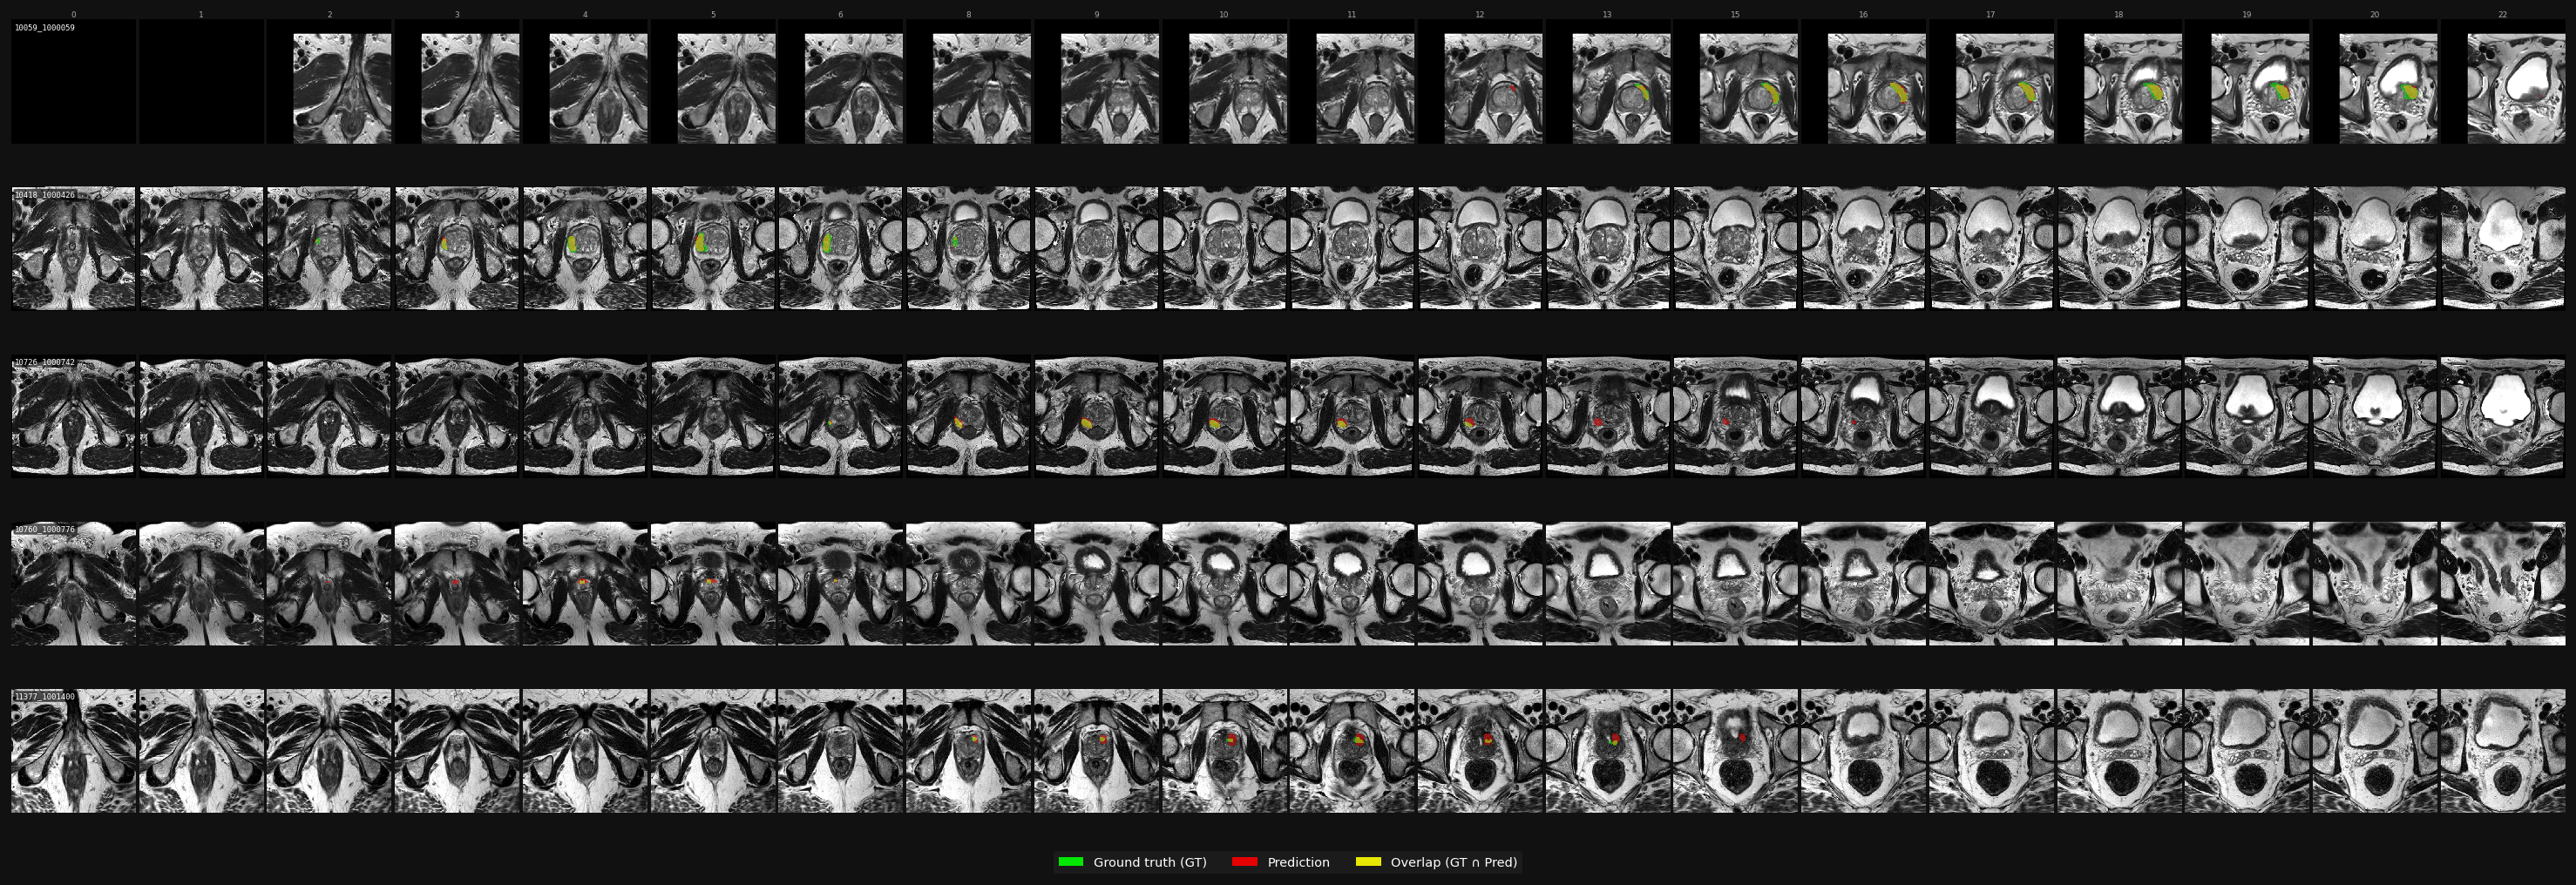
\includegraphics[width=0.78\textwidth]{../visualizations/20260427_221309_unet3d_eval_visualization.png}
\caption{Example qualitative result for the Attention SSL run.}
\end{figure}

\begin{figure}[H]
\centering
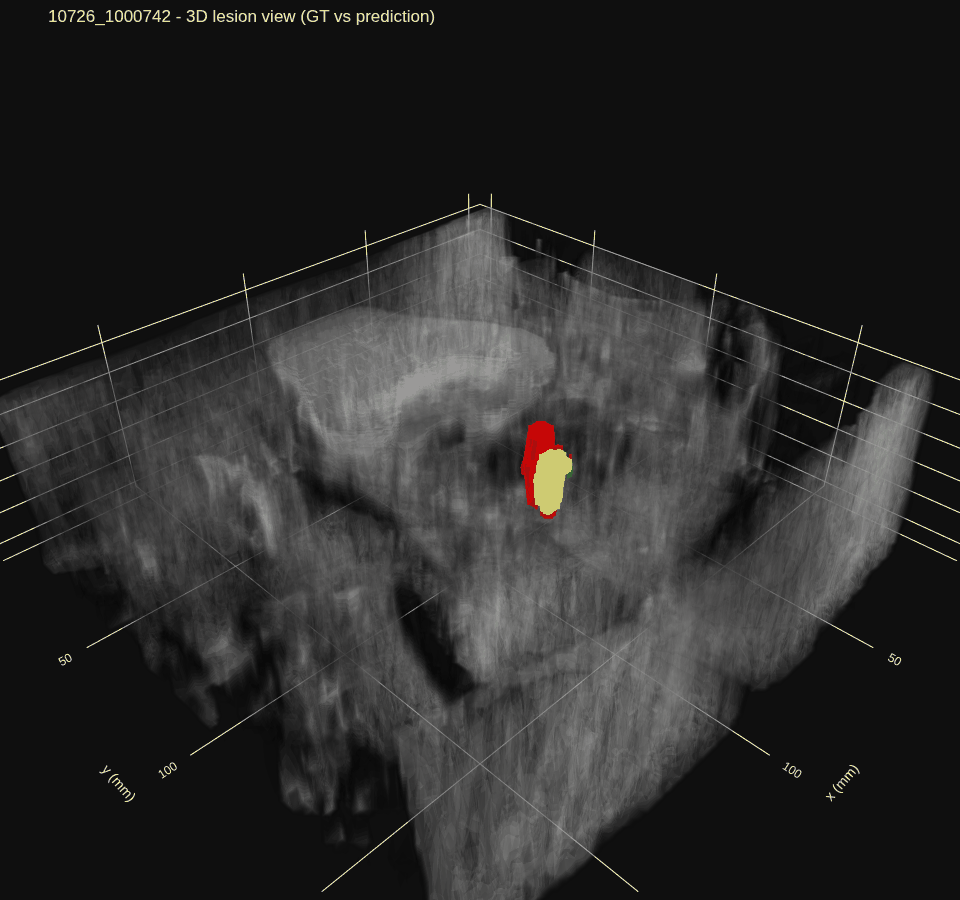
\includegraphics[width=0.78\textwidth]{../visualizations/20260427_221309_unet3d_10726_1000742_t2w_orbit_first_frame.png}
\caption{Example 3D visualization for the Attention SSL run.}
\end{figure}

\subsection{Deconver Runs}

Deconver was introduced as an alternative medical image segmentation architecture with a different feature-mixing mechanism than the Attention U-Net baseline \cite{deconver}. The main goal of these experiments was to test whether this architecture could produce stronger segmentation quality and more stable boundary predictions. The Deconver runs later expanded into a tuned re-run and a multitask variant, so this family now covers both direct baseline comparison and more experimental follow-up work. As with the Attention U-Net section, results are reported both on the fixed 10-case PI-CAI test set and on the 19-case Prostate158 test set whenever both evaluations are available.

\begin{table}[H]
\centering
\scriptsize
\begin{tabular}{>{\raggedright\arraybackslash}p{0.15\textwidth} >{\raggedright\arraybackslash}p{0.20\textwidth} c c c c c c}
\toprule
Run & Main change & P-Dice & P-Sens. & P-HD95 & Pr-Dice & Pr-Sens. & Pr-HD95 \\
\midrule
Deconver baseline & first Deconver baseline & \textbf{0.6470} & 0.7732 & \textbf{3.8062} & 0.4591 & 0.5418 & 18.2104 \\
Deconver ablation & T2w + ADC only, val every 5 epochs & 0.6143 & 0.8629 & 12.8735 & 0.4345 & 0.5652 & 21.9676 \\
Deconver tuned A & tuned schedule and lower learning rate & 0.6452 & 0.7320 & 4.1868 & 0.4703 & 0.4860 & 19.2852 \\
Deconver tuned A + Prostate158 fine-tuning & Prostate158 fine-tuning from tuned A & 0.5030 & \textbf{0.9005} & 99.6676 & 0.4827 & \textbf{0.7158} & 23.1738 \\
Deconver multitask & multitask variant with balanced score & 0.6076 & 0.6686 & 4.7500 & \textbf{0.4899} & 0.4942 & \textbf{16.0527} \\
Deconver tuned A + Prostate158 short fine-tuning & shorter Prostate158 fine-tuning from tuned A & 0.5118 & 0.9002 & 115.9511 & 0.4895 & 0.6913 & 20.6807 \\
\bottomrule
\end{tabular}
\caption{Deconver runs. P = PI-CAI 10-case test set, Pr = Prostate158 19-case test set.}
\normalsize
\end{table}

The two later tuned A descendants were both fine-tuned on Prostate158 starting from the original \textit{Deconver tuned A} checkpoint. The purpose of this fine-tuning was to check whether the model could perform better on the Prostate158 dataset without losing the score that the baseline model had on the initial PI-CAI test set.

\subsubsection*{Detailed Run: Deconver Baseline}

This run represents the first main Deconver baseline. The goal was to compare Deconver directly against the earlier Attention U-Net runs while keeping the multimodal setting with T2w, ADC, and HBV inputs \cite{deconver}. It used the later balanced loss setup and included HD95 during validation.

\begin{table}[H]
\centering
\begin{tabular}{lcc}
\toprule
Metric & PI-CAI (10 cases) & Prostate158 (19 cases) \\
\midrule
Dice & 0.6470 & 0.4591 \\
IoU & 0.4992 & 0.3403 \\
Sensitivity & 0.7732 & 0.5418 \\
Precision & 0.6525 & 0.5582 \\
HD95 & 3.8062 & 18.2104 \\
\bottomrule
\end{tabular}
\caption{Evaluation results for the Deconver baseline run on both test sets.}
\end{table}

\begin{figure}[H]
\centering
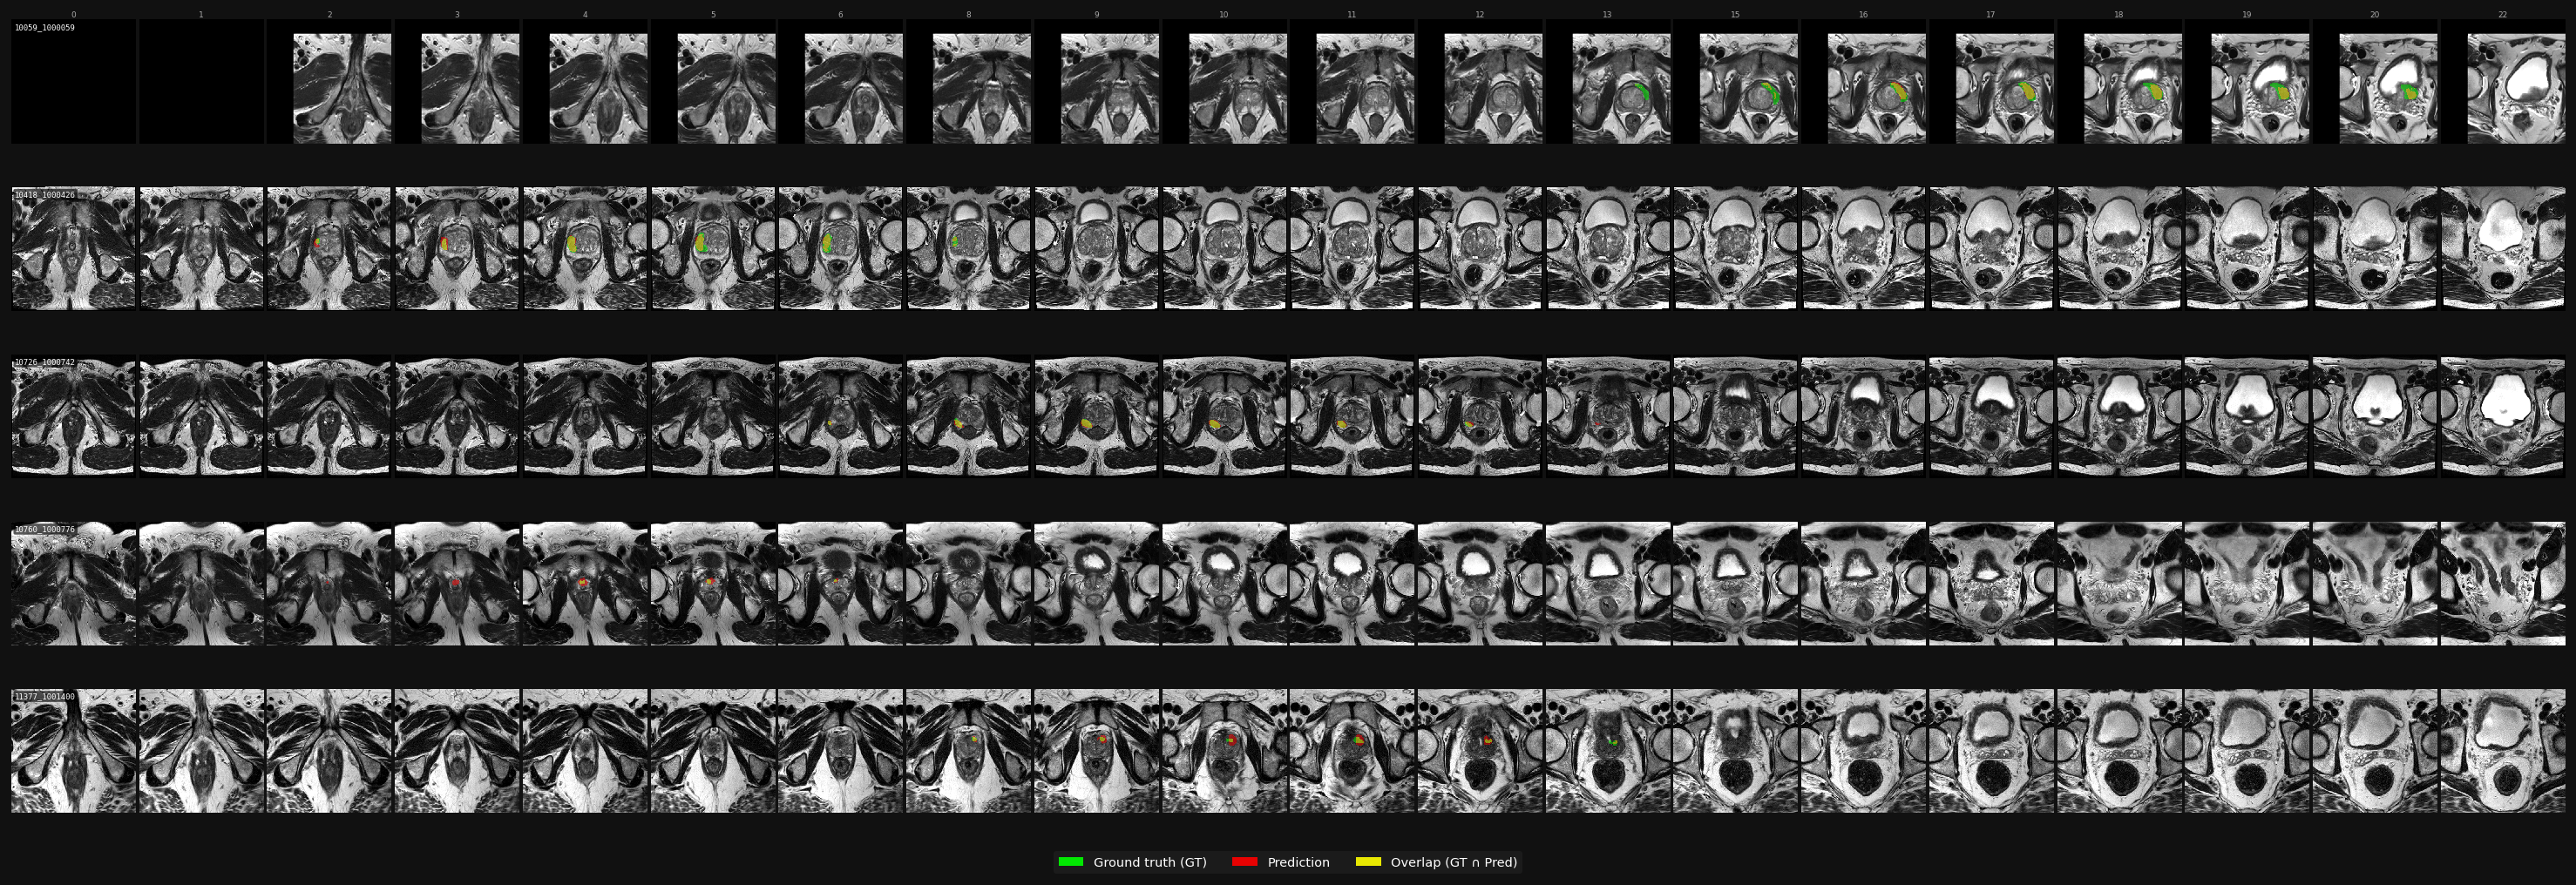
\includegraphics[width=0.78\textwidth]{../visualizations/20260418_224246_deconver_eval_visualization.png}
\caption{Example qualitative result for the Deconver baseline run.}
\end{figure}

\begin{figure}[H]
\centering
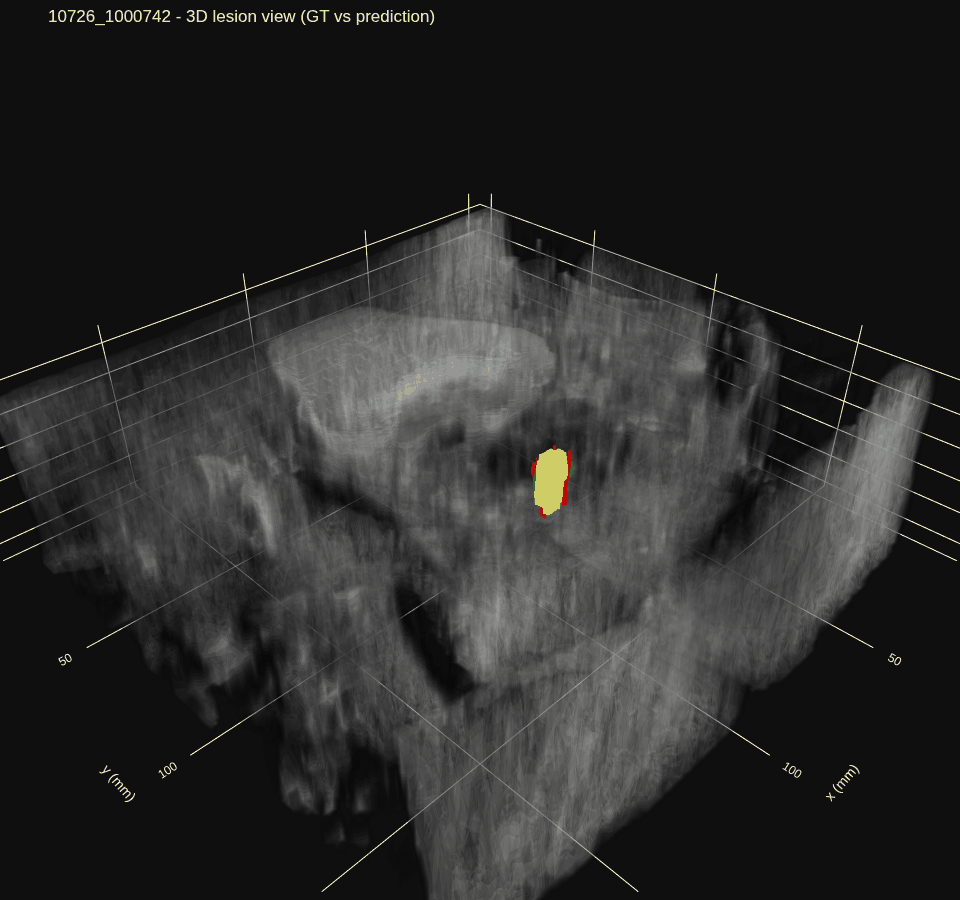
\includegraphics[width=0.78\textwidth]{../visualizations/20260418_224246_deconver_10726_1000742_t2w_orbit_first_frame.png}
\caption{Example 3D visualization for the Deconver baseline run.}
\end{figure}

\subsubsection*{Detailed Run: Deconver Tuned A}

This run represents the main tuned Deconver configuration. Compared to the baseline, it used a lower learning rate, a longer schedule, and a shorter validation warm-up, with the goal of improving training stability and final segmentation quality. It kept the multimodal input setting and remained one of the strongest directly comparable Deconver runs in the report.

\begin{table}[H]
\centering
\begin{tabular}{lcc}
\toprule
Metric & PI-CAI (10 cases) & Prostate158 (19 cases) \\
\midrule
Dice & 0.6452 & 0.4703 \\
IoU & 0.4901 & 0.3442 \\
Sensitivity & 0.7320 & 0.4860 \\
Precision & 0.6810 & 0.5458 \\
HD95 & 4.1868 & 19.2852 \\
\bottomrule
\end{tabular}
\caption{Evaluation results for the Deconver tuned A run on both test sets.}
\end{table}

\begin{figure}[H]
\centering
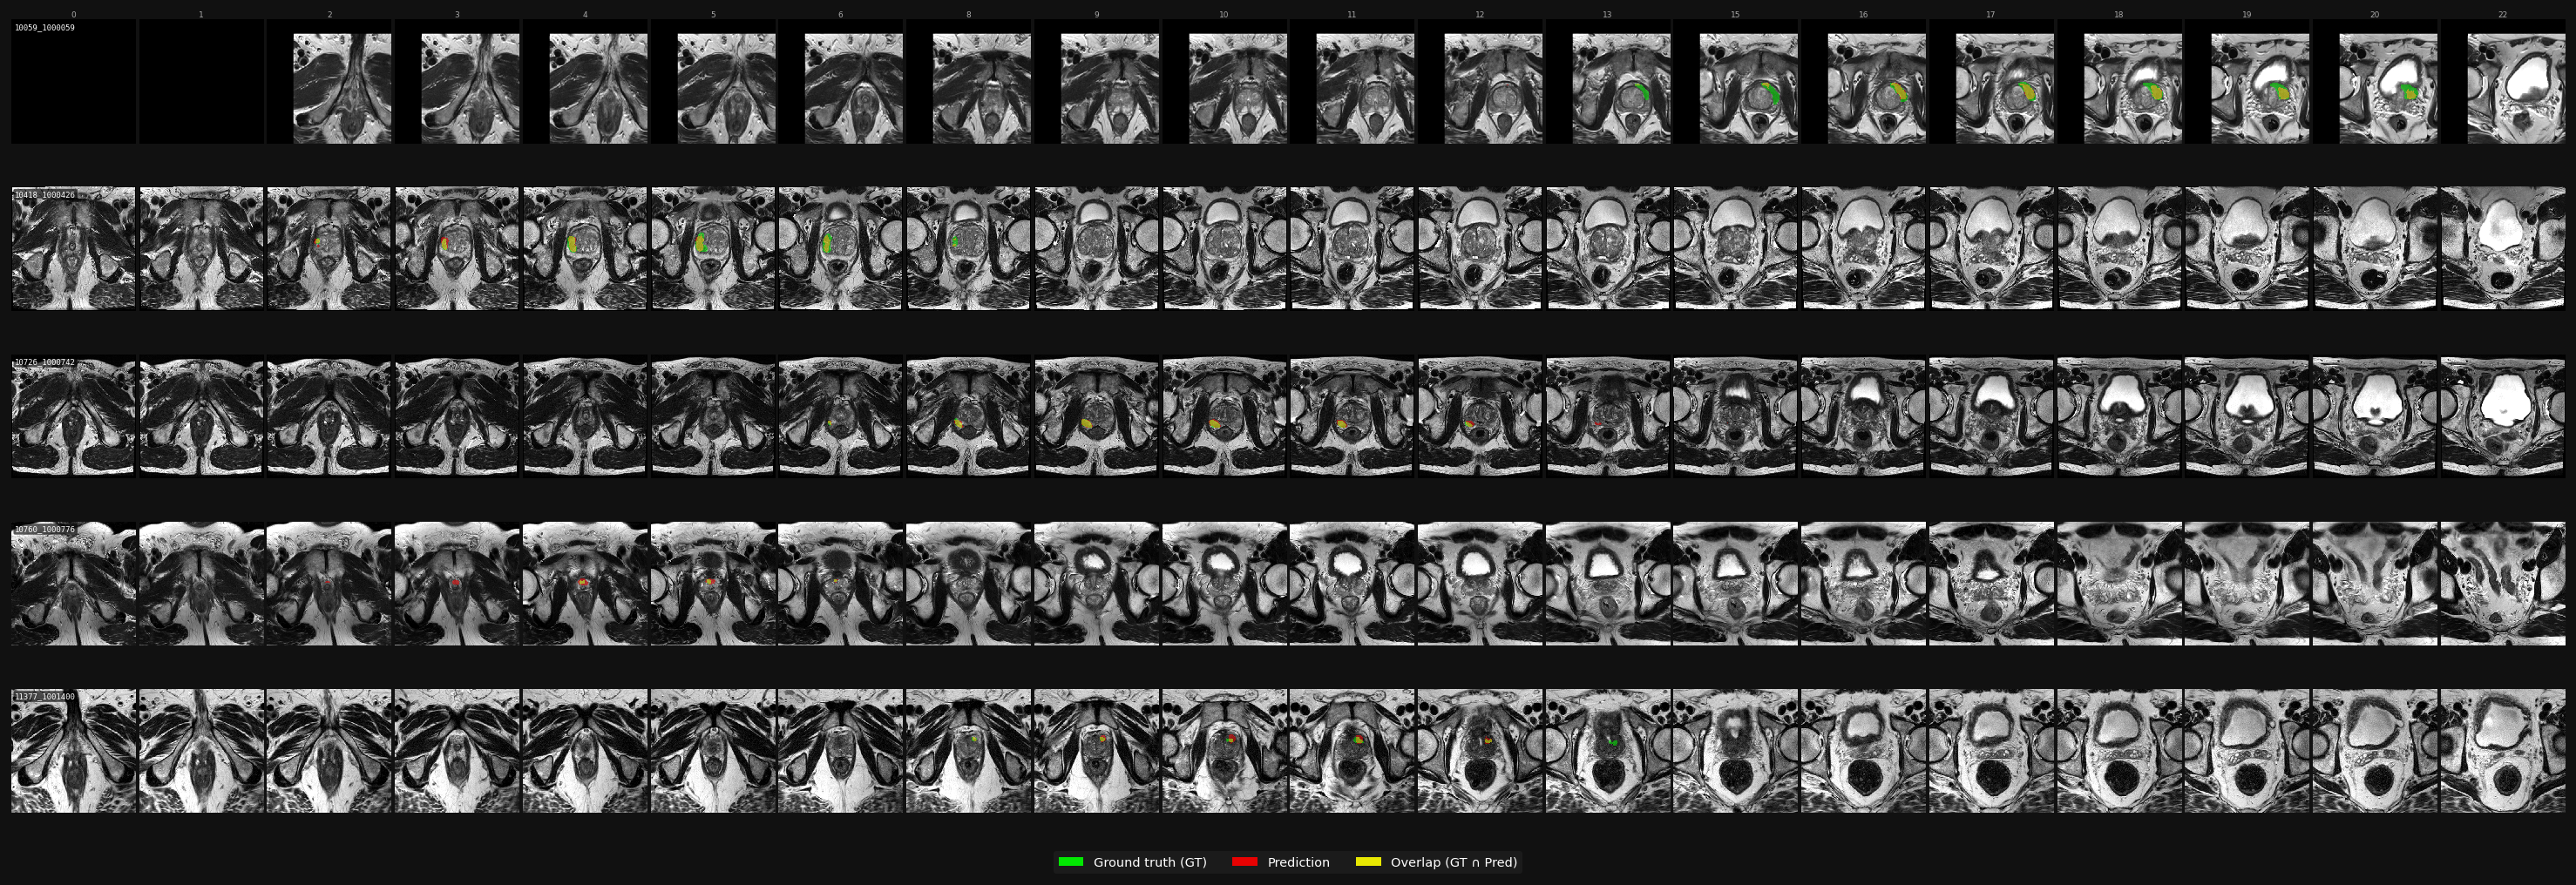
\includegraphics[width=0.78\textwidth]{../visualizations/20260507_193114_deconver_tuned_a_eval_visualization.png}
\caption{Example qualitative result for the Deconver tuned A run.}
\end{figure}

\begin{figure}[H]
\centering
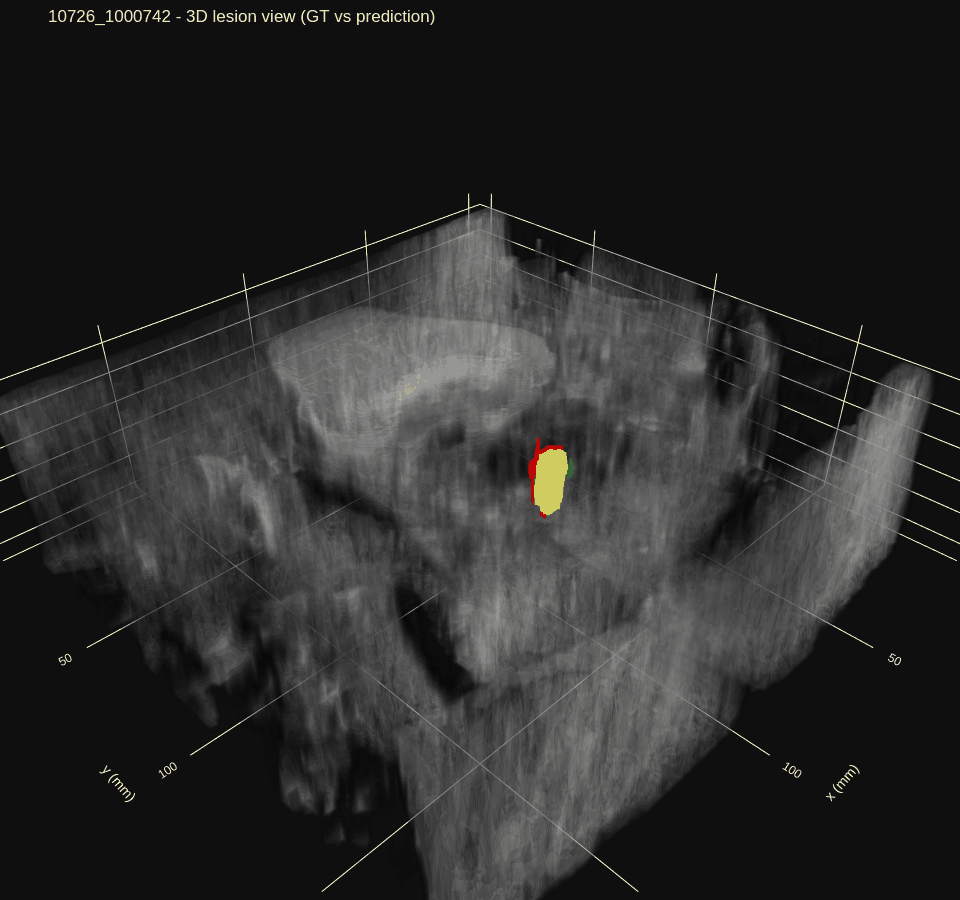
\includegraphics[width=0.78\textwidth]{../visualizations/20260507_193114_deconver_tuned_a_10726_1000742_t2w_orbit_first_frame.png}
\caption{Example 3D visualization for the Deconver tuned A run.}
\end{figure}

\subsubsection*{Detailed Run: Deconver Multitask}

This run tested the multitask Deconver variant with a balanced score setup. The main goal was to check whether the multitask formulation could reduce false positives while keeping competitive segmentation performance on the evaluation sets.

\begin{table}[H]
\centering
\begin{tabular}{lcc}
\toprule
Metric & PI-CAI (10 cases) & Prostate158 (19 cases) \\
\midrule
Dice & 0.6076 & 0.4899 \\
IoU & 0.4557 & 0.3577 \\
Sensitivity & 0.6686 & 0.4942 \\
Precision & 0.6985 & 0.6104 \\
HD95 & 4.7500 & 16.0527 \\
\bottomrule
\end{tabular}
\caption{Evaluation results for the Deconver multitask run on both test sets.}
\end{table}

\begin{figure}[H]
\centering
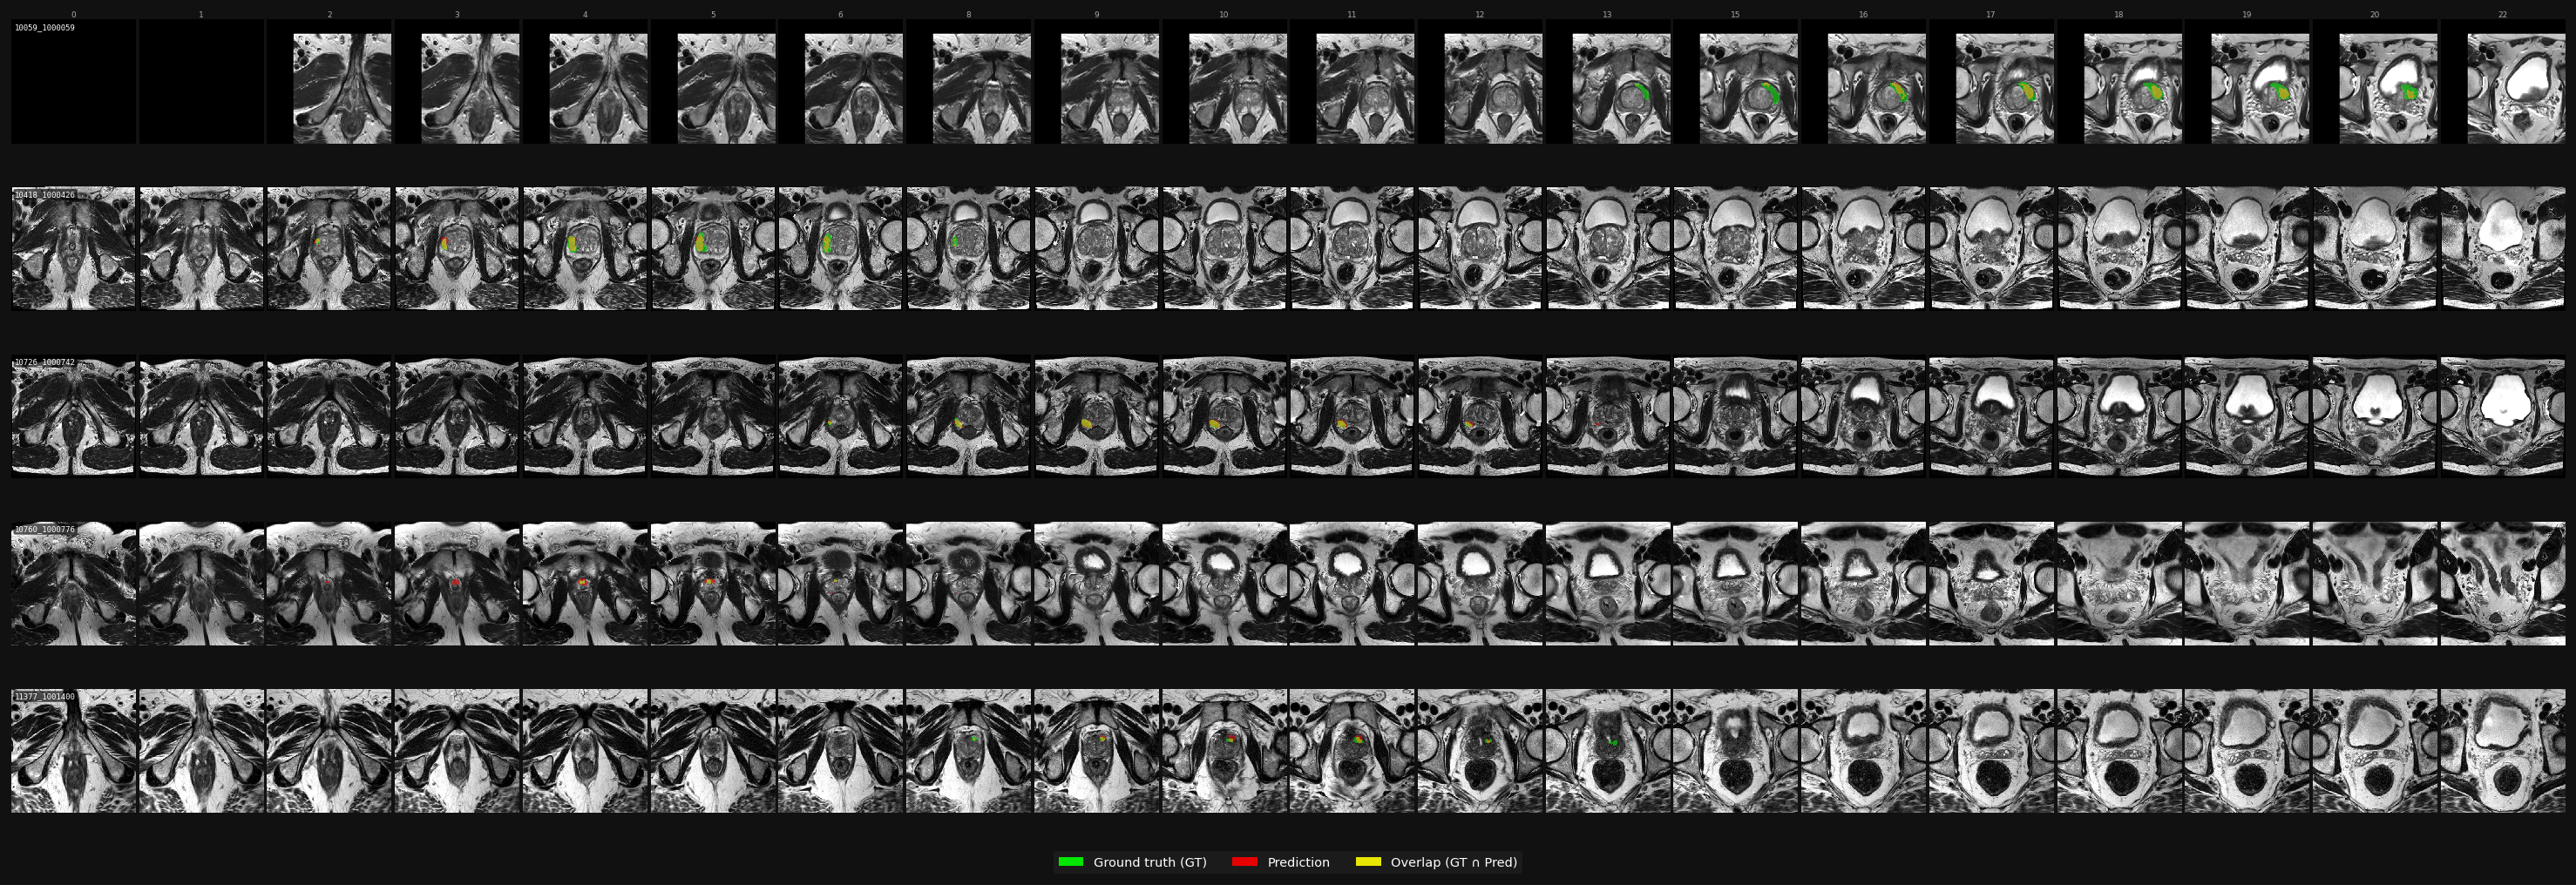
\includegraphics[width=0.78\textwidth]{../visualizations/20260513_105631_deconver_multitask_a_eval_visualization.png}
\caption{Example qualitative result for the Deconver multitask run.}
\end{figure}

\begin{figure}[H]
\centering
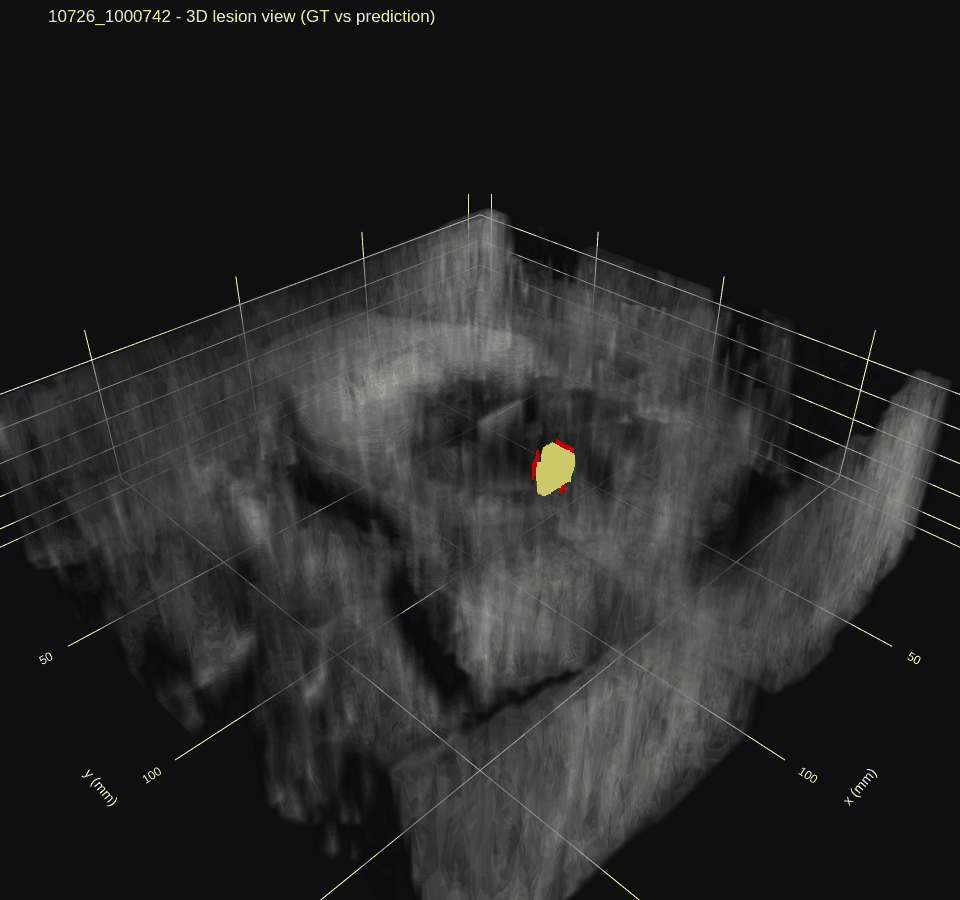
\includegraphics[width=0.78\textwidth]{../visualizations/20260513_105631_deconver_multitask_a_10726_1000742_t2w_orbit_first_frame.png}
\caption{Example 3D visualization for the Deconver multitask run.}
\end{figure}

\subsection{FCT Run}

FCT was added because I wanted to test a vision-transformer-based approach, but standard vision transformers are computationally expensive for this type of segmentation task. Because of that, I looked for more practical alternatives and chose a convolutional vision transformer style model \cite{cvt}. The original FCT method was proposed for 2D medical image segmentation \cite{fct}, and the original work did not test it on 3D volumes. For this project, I adapted it to the 3D pipeline by processing volumetric MRI inputs slice-wise with a 2D FCT encoder-decoder and then stacking the slice predictions back into a 3D output volume. This made it suitable for comparison with the Attention U-Net and Deconver models used in this work. As in the previous sections, results are reported both on the fixed 10-case PI-CAI test set and on the 19-case Prostate158 test set.

\begin{table}[H]
\centering
\scriptsize
\begin{tabular}{>{\raggedright\arraybackslash}p{0.18\textwidth} >{\raggedright\arraybackslash}p{0.20\textwidth} c c c c c c}
\toprule
Run & Main change & P-Dice & P-Sens. & P-HD95 & Pr-Dice & Pr-Sens. & Pr-HD95 \\
\midrule
FCT baseline & transformer-based baseline & \textbf{0.5780} & \textbf{0.5308} & \textbf{4.4900} & \textbf{0.4079} & \textbf{0.4143} & \textbf{34.3002} \\
\bottomrule
\end{tabular}
\caption{FCT run summary. P = PI-CAI 10-case test set, Pr = Prostate158 19-case test set.}
\normalsize
\end{table}

\subsubsection*{Detailed Run: FCT Baseline}

This run used the FCT architecture with multimodal T2w, ADC, and HBV input \cite{fct}. The main reason for including it was to test a transformer-inspired model without using a full vision transformer, which would be slower and more computationally demanding. Since FCT was originally designed for 2D segmentation rather than 3D MRI volumes, I converted it for this project into a slice-wise model: each axial slice was processed with a 2D FCT encoder-decoder, and the resulting slice predictions were combined back into a volumetric segmentation output. This provided a practical way to compare this type of architecture against the CNN-based and Deconver-based models.

\begin{table}[H]
\centering
\begin{tabular}{lcc}
\toprule
Metric & PI-CAI (10 cases) & Prostate158 (19 cases) \\
\midrule
Dice & 0.5780 & 0.4079 \\
IoU & 0.4217 & 0.3099 \\
Sensitivity & 0.5308 & 0.4143 \\
Precision & 0.6968 & 0.5898 \\
HD95 & 4.4900 & 34.3002 \\
\bottomrule
\end{tabular}
\caption{Evaluation results for the FCT baseline run on both test sets.}
\end{table}

\begin{figure}[H]
\centering
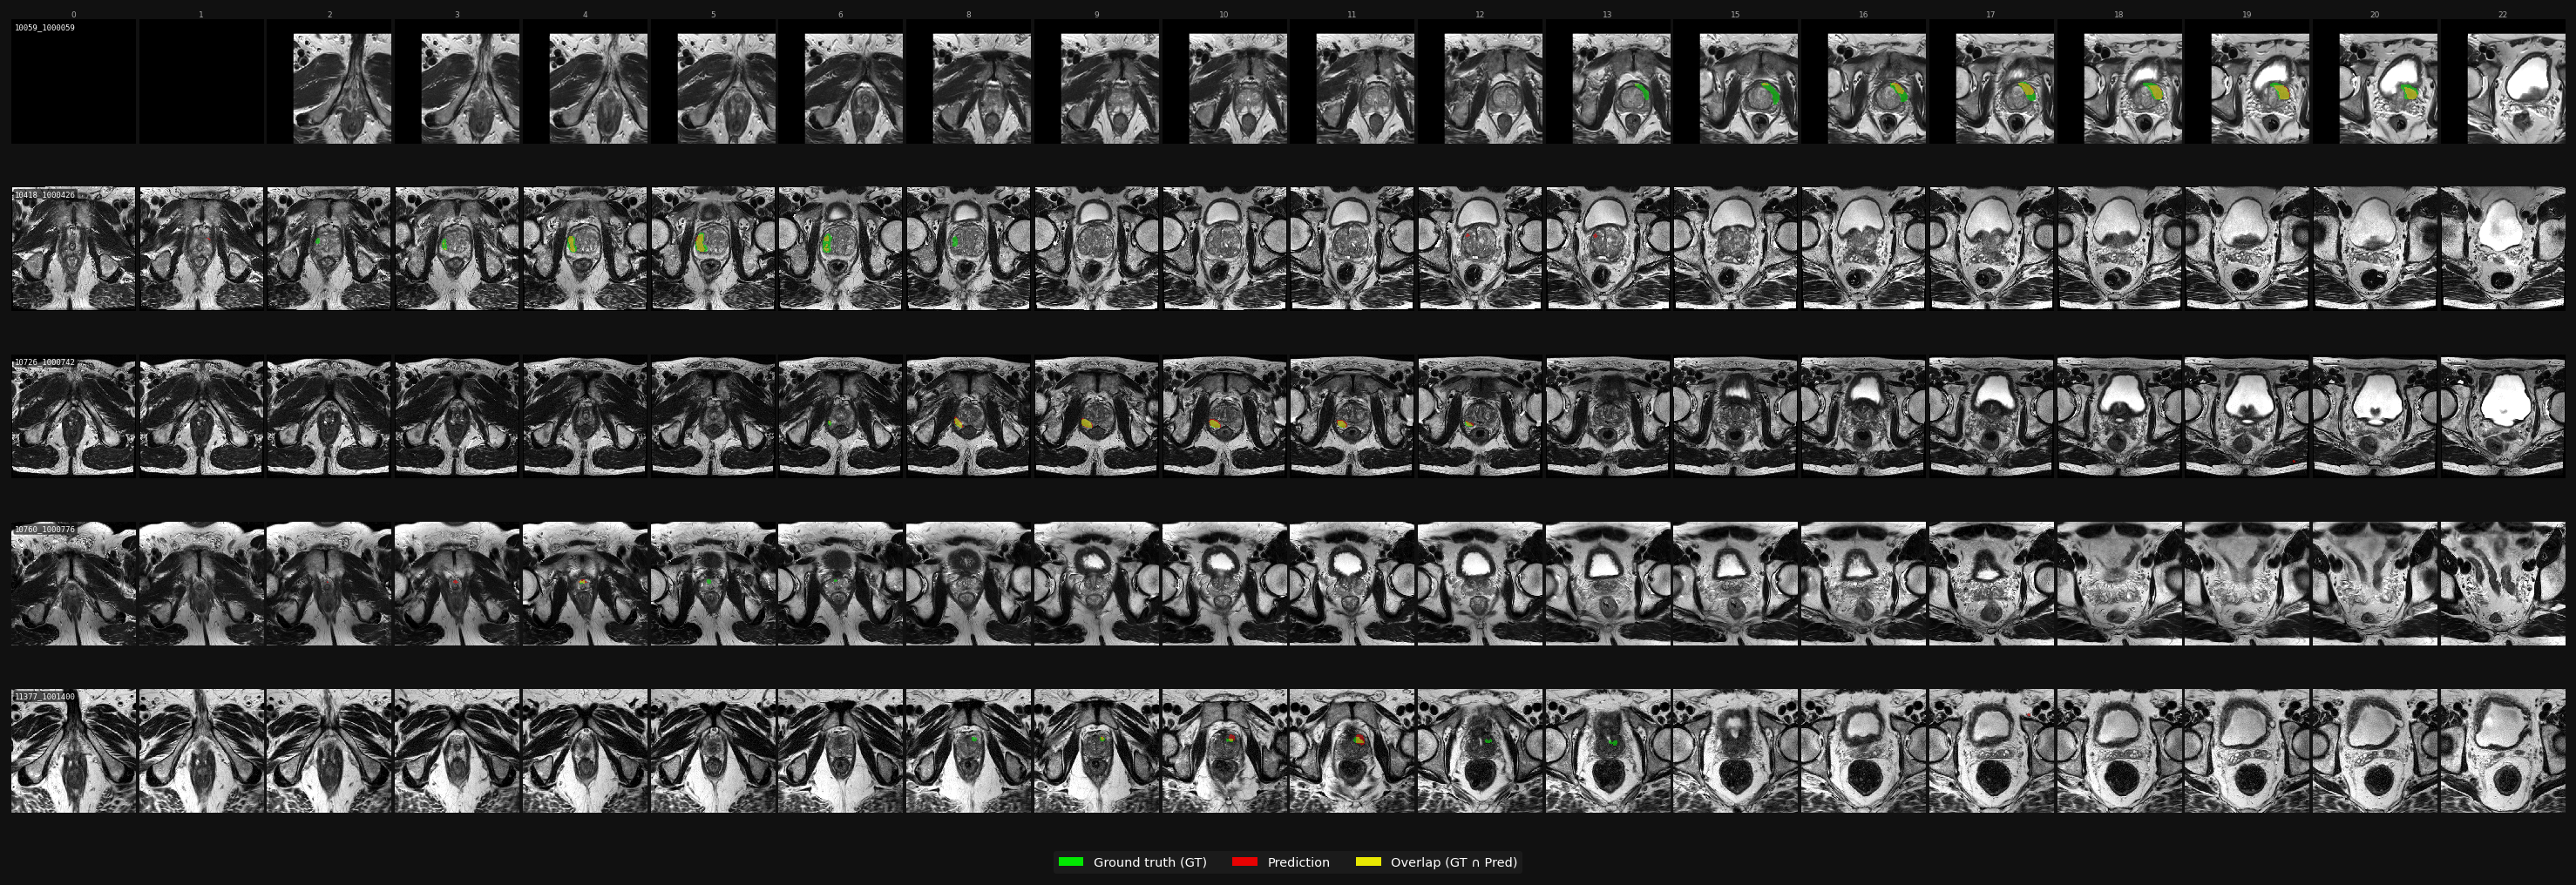
\includegraphics[width=0.78\textwidth]{../visualizations/20260507_205845_fct_default_eval_visualization.png}
\caption{Example qualitative result for the FCT run.}
\end{figure}

\begin{figure}[H]
\centering
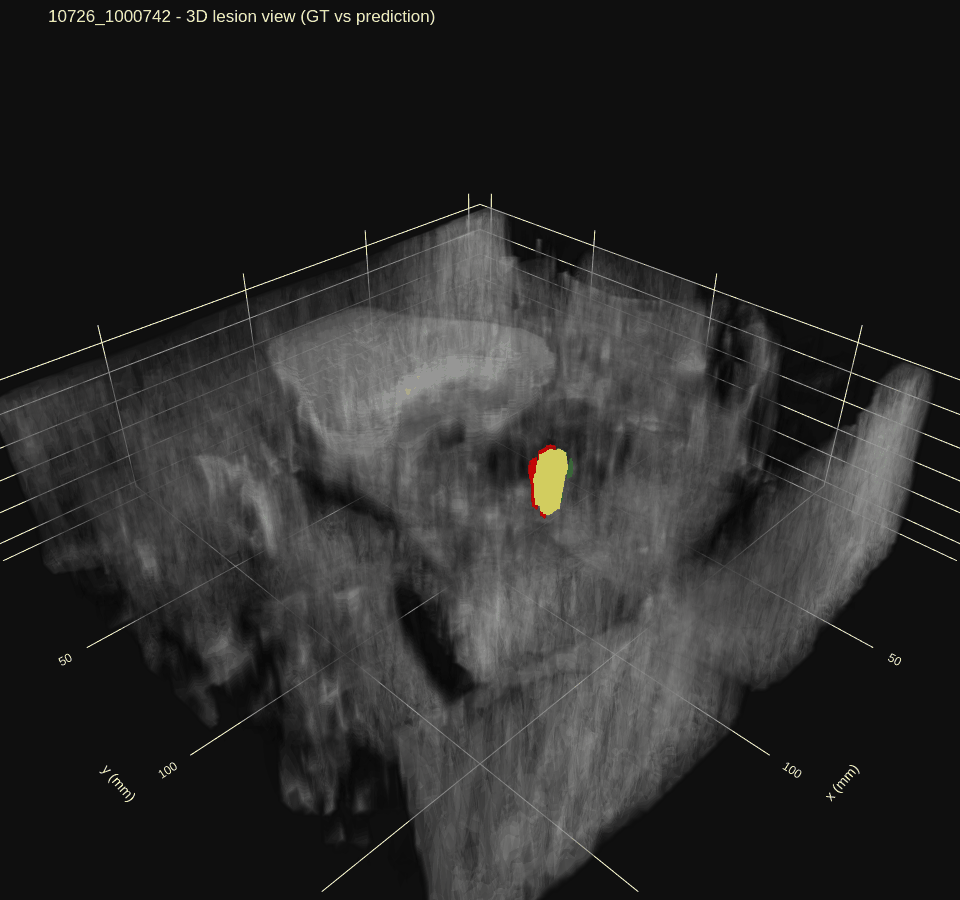
\includegraphics[width=0.78\textwidth]{../visualizations/20260507_205845_fct_default_10726_1000742_t2w_orbit_first_frame.png}
\caption{Example 3D visualization for the FCT run.}
\end{figure}

\subsection{Cross-Model Comparison}

This section summarizes the main differences between the most representative runs that share the same fixed PI-CAI 10-case evaluation setup.

\begin{table}[H]
\centering
\begin{tabular}{>{\raggedright\arraybackslash}p{0.30\textwidth} c c c c}
\toprule
Run & Comp. & Dice & Sens. & HD95 \\
\midrule
Attention SSL run & 0.4409 & 0.6332 & \textbf{0.8329} & 4.4875 \\
Deconver baseline & 0.4709 & \textbf{0.6470} & 0.7732 & \textbf{3.8062} \\
Deconver tuned A & \textbf{0.4772} & 0.6452 & 0.7320 & 4.1868 \\
FCT baseline & 0.4311 & 0.5780 & 0.5308 & 4.4900 \\
\bottomrule
\end{tabular}
\caption{Compact comparison of the main representative runs on the fixed PI-CAI 10-case test set.}
\end{table}

Overall, the Deconver family currently looks strongest in this report. The Deconver baseline gave the best PI-CAI Dice and the lowest HD95, while Deconver tuned A kept nearly the same segmentation quality together with the best training composite score among the directly comparable representative runs. The Attention SSL run remained competitive and achieved the highest sensitivity, while FCT was useful as a transformer-based comparison but did not match the strongest Deconver or Attention results across both evaluation sets.

\section{Explainable AI (XAI)}

XAI was added to check whether the models relied on the lesion region and the imaging channels that are clinically relevant for prostate MRI \cite{xai_survey}. Segmentation scores alone do not show if a model is using sensible cues or if it is leaning on shortcuts in the image. The explanation methods therefore served as a sanity check on the learned behaviour.

\subsection{Methods Used}

The main XAI methods used in this work are:
\begin{itemize}
    \item \textbf{Grad-CAM} -- gives a coarse map of the regions that most influence the prediction,
    \item \textbf{Saliency maps} -- show which voxels or channels have the strongest effect on the output,
    \item \textbf{Modality ablation} -- measures how the prediction changes when one input modality is removed.
\end{itemize}

These methods were kept simple and practical so they could be compared across model families.

The Deconver baseline is shown here as a representative XAI example because it is one of the strongest runs in the report and already has a complete set of XAI outputs.

\begin{figure}[H]
\centering
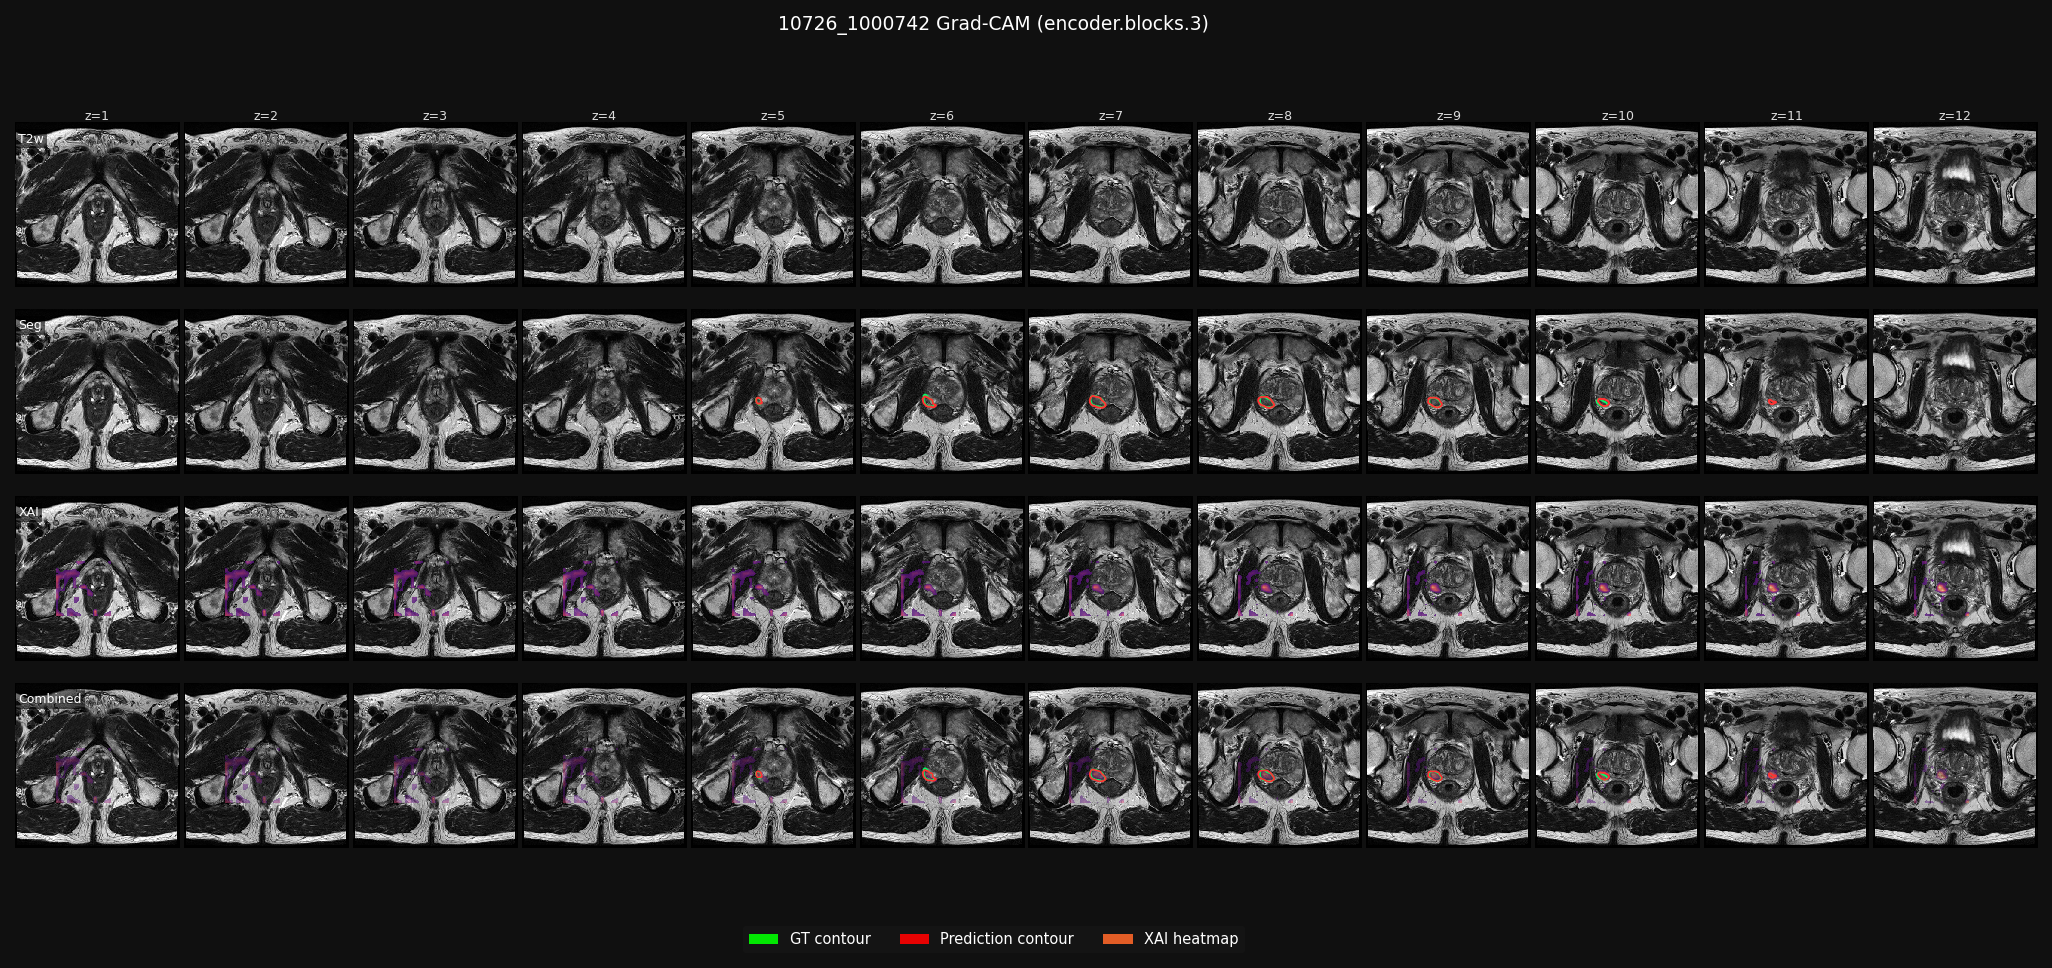
\includegraphics[width=0.78\textwidth]{../visualizations/xai/20260418_224246_deconver_10726_1000742_gradcam.png}
\caption{Deconver baseline XAI example using Grad-CAM.}
\end{figure}

\begin{figure}[H]
\centering
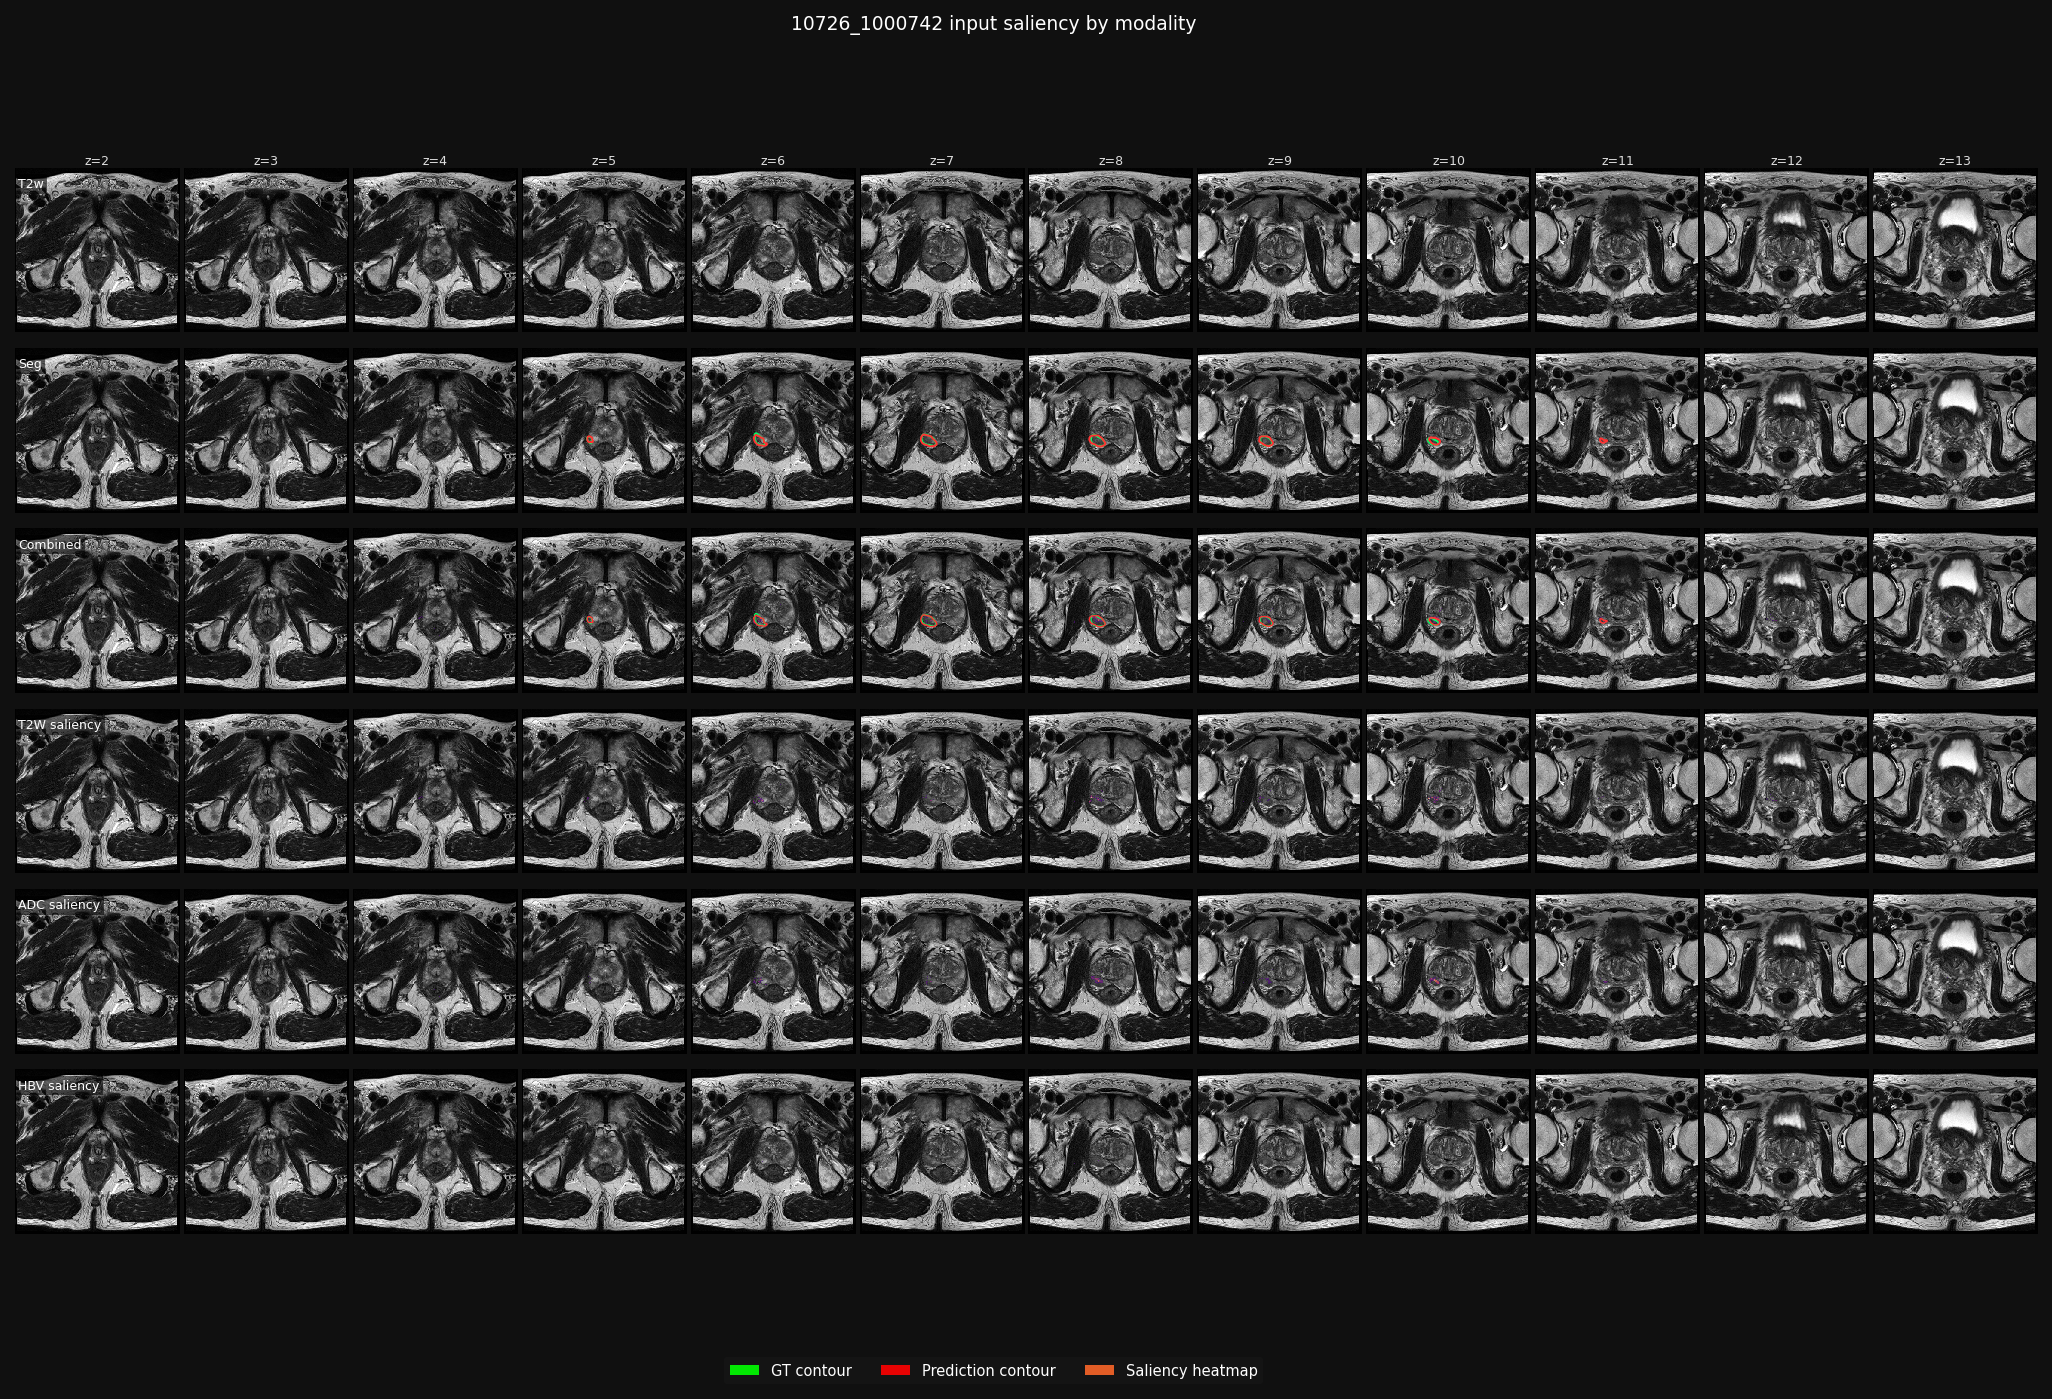
\includegraphics[width=0.78\textwidth]{../visualizations/xai/20260418_224246_deconver_10726_1000742_saliency.png}
\caption{Deconver baseline XAI example using combined saliency maps.}
\end{figure}

\begin{figure}[H]
\centering
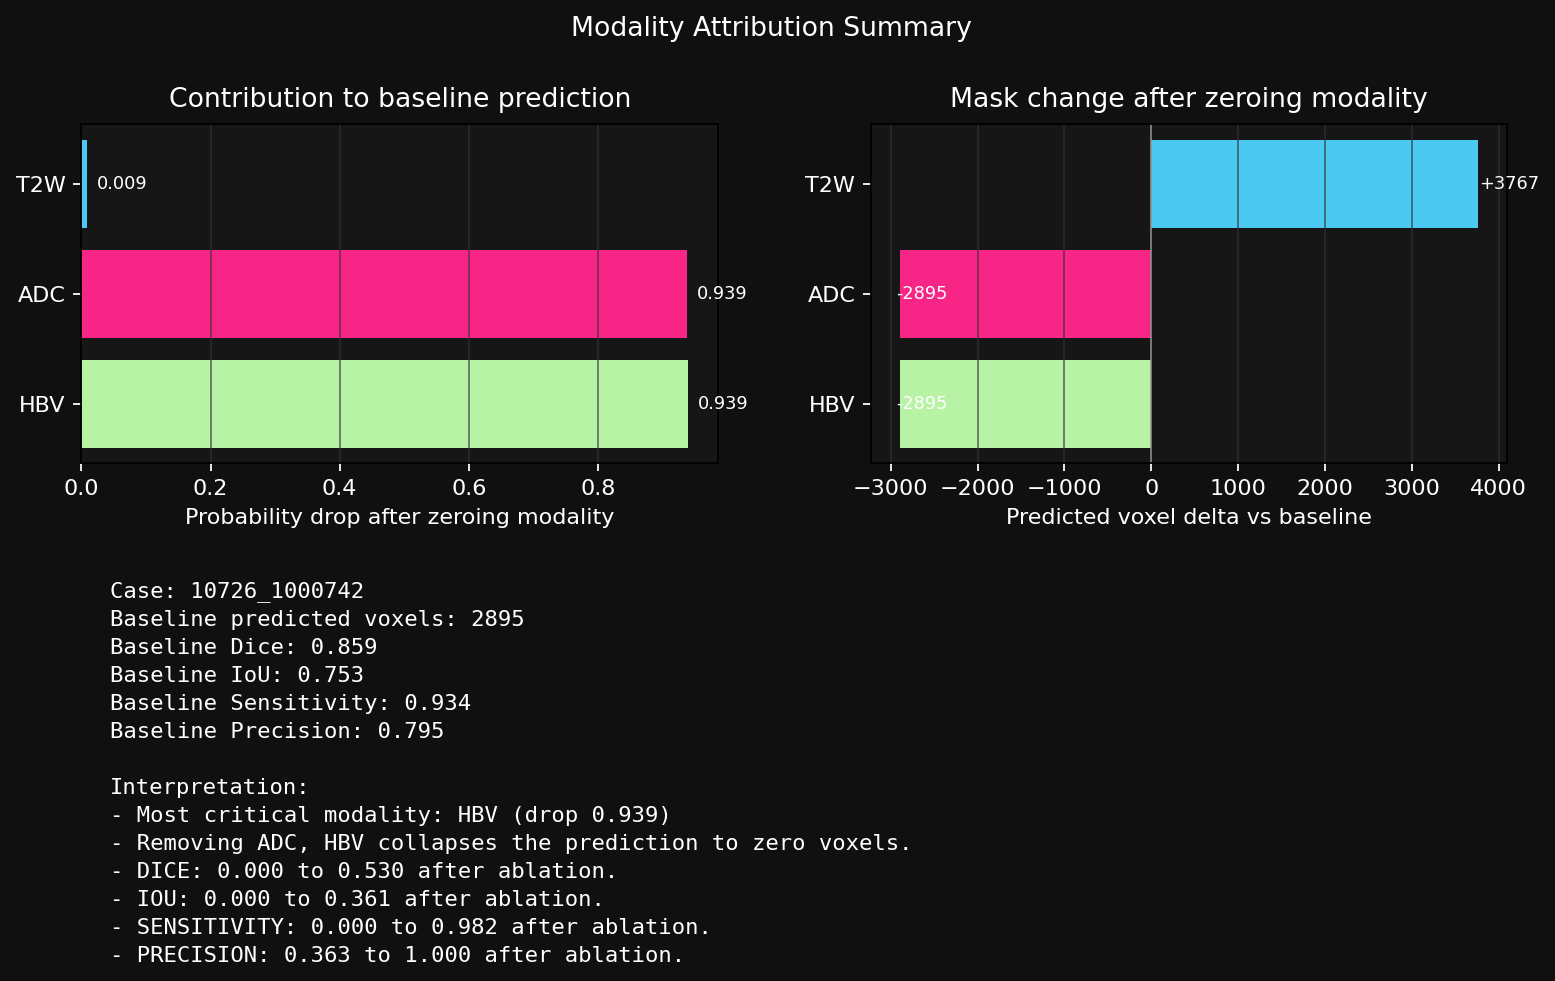
\includegraphics[width=0.78\textwidth]{../visualizations/xai/20260418_224246_deconver_10726_1000742_modality_ablation_summary.png}
\caption{Deconver baseline XAI example using modality ablation.}
\end{figure}

\section{General Discussion}

Deconver currently looks like the strongest model family in this report. Deconver tuned A gave the best PI-CAI Dice and one of the best HD95 values, while the later Prostate158 fine-tuning runs achieved high sensitivity but did not improve the final PI-CAI boundary quality. The Attention SSL run remained competitive and reached the highest sensitivity, but its HD95 and precision were less stable. FCT was a useful transformer-style comparison, but it did not surpass the best CNN-based runs. The main limitations are the small fixed PI-CAI test set, the modest external Prostate158 test set, and the fact that validation composite score does not always track final test quality.

\section{Future Work and Ideas}

\begin{itemize}
    \item Experiment more with multitask models.
    \item Use the Prostate158 prostate segmentation masks to test a two-stage cascade, where the first stage defines the ROI and the second stage performs lesion segmentation.
    \item Try implementing a diffusion model based on the approach in \cite{segdiff}.
\end{itemize}

\begin{thebibliography}{99}

\bibitem{deconver}
P. Ashtari, S. Noei, F. Nateghi Haredasht, J. H. Chen, G. Jurman, A. Pizurica, and S. Van Huffel,
``Deconver: A Deconvolutional Network for Medical Image Segmentation,''
\href{https://arxiv.org/abs/2504.00302}{arXiv:2504.00302}, 2025. \href{https://doi.org/10.48550/arXiv.2504.00302}{doi:10.48550/arXiv.2504.00302}.

\bibitem{fct}
A. Tragakis, C. Kaul, R. Murray-Smith, and D. Husmeier,
``The Fully Convolutional Transformer for Medical Image Segmentation,''
in \textit{Proceedings of the IEEE/CVF Winter Conference on Applications of Computer Vision (WACV)},
pp. 3660--3669, 2023. \href{https://arxiv.org/abs/2206.00566}{arXiv:2206.00566}. \href{https://doi.org/10.48550/arXiv.2206.00566}{doi:10.48550/arXiv.2206.00566}.

\bibitem{cvt}
H. Wu, B. Xiao, N. Codella, M. Liu, X. Dai, L. Yuan, and L. Zhang,
``CvT: Introducing Convolutions to Vision Transformers,''
\href{https://arxiv.org/abs/2103.15808}{arXiv:2103.15808}, 2021. \href{https://doi.org/10.48550/arXiv.2103.15808}{doi:10.48550/arXiv.2103.15808}.

\bibitem{picai_dataset}
A. Saha, J. J. Twilt, J. S. Bosma, B. van Ginneken, D. Yakar, M. Elschot, J. Veltman, J. F\"utterer, M. de Rooij, and H. Huisman,
``The PI-CAI Challenge: Public Training and Development Dataset,''
\href{https://zenodo.org/records/6624726}{Zenodo}, version v2.0, 2022. \href{https://doi.org/10.5281/zenodo.6624726}{doi:10.5281/zenodo.6624726}.

\bibitem{prostate158_main}
L. C. Adams, M. R. Makowski, G. Engel, M. Rattunde, F. Busch, P. Asbach, S. M. Niehues, S. Vinayahalingam, B. van Ginneken, G. Litjens, and K. K. Bressem,
``Prostate158 - An expert-annotated 3T MRI dataset and algorithm for prostate cancer detection,''
\textit{Computers in Biology and Medicine}, vol. 148, p. 105817, 2022. \href{https://doi.org/10.1016/j.compbiomed.2022.105817}{doi:10.1016/j.compbiomed.2022.105817}.

\bibitem{prostate158_dib}
L. C. Adams, M. R. Makowski, G. Engel, M. Rattunde, F. Busch, P. Asbach, S. M. Niehues, S. Vinayahalingam, B. van Ginneken, G. Litjens, and K. K. Bressem,
``Dataset of prostate MRI annotated for anatomical zones and cancer,''
\textit{Data in Brief}, vol. 45, p. 108739, 2022. \href{https://doi.org/10.1016/j.dib.2022.108739}{doi:10.1016/j.dib.2022.108739}.

\bibitem{xai_survey}
F. Xu, H. Uszkoreit, Y. Du, W. Fan, D. Zhao, and J. Zhu,
``Explainable AI: A Brief Survey on History, Research Areas, Approaches and Challenges,''
in \textit{NLPCC 2019}, pp. 563--574, 2019. \href{https://doi.org/10.1007/978-3-030-32236-6_51}{doi:10.1007/978-3-030-32236-6\_51}.

\bibitem{segdiff}
T. Amit, T. Shaharbany, E. Nachmani, and L. Wolf,
``SegDiff: Image Segmentation with Diffusion Probabilistic Models,''
\href{https://arxiv.org/abs/2112.00390}{arXiv:2112.00390}, 2022. \href{https://doi.org/10.48550/arXiv.2112.00390}{doi:10.48550/arXiv.2112.00390}.

\bibitem{medsegdiff}
J. Wu, R. Fu, H. Fang, Y. Zhang, Y. Yang, H. Xiong, H. Liu, and Y. Xu,
``MedSegDiff: Medical Image Segmentation with Diffusion Probabilistic Model,''
\href{https://arxiv.org/abs/2211.00611}{arXiv:2211.00611}, 2023. \href{https://doi.org/10.48550/arXiv.2211.00611}{doi:10.48550/arXiv.2211.00611}.

\end{thebibliography}

\end{document}
